%  LaTeX support: latex@mdpi.com
%  For support, please attach all files needed for compiling as well as the log file, and specify your operating system, LaTeX version, and LaTeX editor.

% Teruskan opsi [numbers] ke natbib sebelum class memuatnya (hindari option clash):
\PassOptionsToPackage{numbers}{natbib}
%=================================================================
\documentclass[metlit,article,accept,pdftex,moreauthors]
{Definitions/mdpi}
\usepackage{caption} % Catatan: caption sudah dimuat oleh class mdpi; baris ini dipertahankan untuk kompatibilitas subcaption.
\usepackage{subcaption}
\usepackage[indonesian]{babel}
% \usepackage[numbers]{natbib} % Dimuat oleh class mdpi; opsi diteruskan via \PassOptionsToPackage di atas.
\usetikzlibrary{shapes.geometric, arrows.meta, positioning}
% \linenumbers
%--------------------

%---------
% pdftex
%---------
% The option pdftex is for use with pdfLaTeX. Remove "pdftex" for (1) compiling with LaTeX & dvi2pdf (if eps figures are used) or for (2) compiling with XeLaTeX.

%=================================================================
% MDPI internal commands - do not modify
\firstpage{1}
\makeatletter
\setcounter{page}{\@firstpage}
\makeatother
\pubvolume{1}
\issuenum{1}
\articlenumber{0}
\pubyear{2024}
\copyrightyear{2024}
%\externaleditor{Academic Editor: Firstname Lastname}
\datereceived{ }
\daterevised{ } % Comment out if no revised date
\dateaccepted{ }
\datepublished{ }
%\datecorrected{} % For corrected papers: "Corrected: XXX" date in the original paper.
%\dateretracted{} % For corrected papers: "Retracted: XXX" date in the original paper.
\hreflink{https://doi.org/} % If needed use \linebreak
%\doinum{}
%\pdfoutput=1 % Uncommented for upload to arXiv.org
%\CorrStatement{yes}  % For updates


%=================================================================
% Add packages and commands here. The following packages are loaded in our class file: fontenc, inputenc, calc, indentfirst, fancyhdr, graphicx, epstopdf, lastpage, ifthen, float, amsmath, amssymb, lineno, setspace, enumitem, mathpazo, booktabs, titlesec, etoolbox, tabto, xcolor, colortbl, soul, multirow, microtype, tikz, totcount, changepage, attrib, upgreek, array, tabularx, pbox, ragged2e, tocloft, marginnote, marginfix, enotez, amsthm, natbib, hyperref, cleveref, scrextend, url, geometry, newfloat, caption, draftwatermark, seqsplit
% cleveref: load \crefname definitions after \begin{document}

%=================================================================
% Please use the following mathematics environments: Theorem, Lemma, Corollary, Proposition, Characterization, Property, Problem, Example, ExamplesandDefinitions, Hypothesis, Remark, Definition, Notation, Assumption
%% For proofs, please use the proof environment (the amsthm package is loaded by the MDPI class).

%=================================================================
% Full title of the paper (Capitalized)
\Title{
Evaluasi Performa Prediksi Probabilistik pada Klasifikasi Kualitas Air Menggunakan Algoritma Natural Gradient Boosting (NGBoost)}

% MDPI internal command: Title for citation in the left column
\TitleCitation{NGBoost untuk Prediksi Probabilistik Kualitas Air}

% Author Orchid ID: enter ID or remove command
\newcommand{\orcidauthorA}{0000-0000-0000-000X} % Add \orcidA{} behind the author's name
%\newcommand{\orcidauthorB}{0000-0000-0000-000X} % Add \orcidB{} behind the author's name

% Authors, for the paper (add full first names)
\Author{Aflah Zaki Siregar$^{1}$, Siti Zahrotul Fajriyah, S.Kom., M.Kom.$^{2}$}

%\longauthorlist{yes}

% MDPI internal command: Authors, for metadata in PDF
\AuthorNames{Aflah Zaki Siregar dan Siti Zahrotul Fajriyah}

% MDPI internal command: Authors, for citation in the left column
\AuthorCitation{Siregar, A.Z.; Fajriyah, S.Z.}
% If this is a Chicago style journal: Lastname, Firstname, Firstname Lastname, and Firstname Lastname.

% Affiliations / Addresses (Add [1] after \address if there is only one affiliation.)
\address{%
$^{1}$ \quad Teknologi Informasi, Telkom University, Bandung, Indonesia\\
$^{2}$ \quad Informatika, Telkom University, Bandung, Indonesia\\
}

% Contact information of the corresponding author
\corres{Correspondence: aflahzaki@student.telkomuniversity.ac.id}

% Current address and/or shared authorship
\firstnote{Alamat saat ini: Jakarta, Setiabudi.}  % Current address should not be the same as any items in the Affiliation section.
\secondnote{Semua penulis telah berkontribusi.}
% The commands \thirdnote{} till \eighthnote{} are available for further notes

%\simplesumm{} % Simple summary

%\conference{} % An extended version of a conference paper

% Abstract (Do not insert blank lines, i.e. \\)
\abstract{Pendekatan \textit{machine learning} deterministik yang dominan pada domain kualitas air hanya menghasilkan prediksi titik tunggal (\textit{point estimate}) tanpa mengkuantifikasi ketidakpastian inheren yang melekat pada data parameter fisikokimia. Penelitian ini mengusulkan kerangka kerja prediksi probabilistik berbasis \textit{Natural Gradient Boosting} (NGBoost) untuk klasifikasi kelayakan air minum menggunakan \textit{Water Potability Dataset} (3.276 sampel, 9 parameter fisikokimia). NGBoost memodelkan distribusi penuh probabilitas melalui parameterisasi distribusi Bernoulli dan optimasi berbasis \textit{Natural Gradient} pada \textit{Fisher Information Matrix}, sehingga mampu mengkuantifikasi ketidakpastian prediksi secara eksplisit. Pra-pemrosesan data mencakup imputasi nilai hilang menggunakan MICE (\textit{Multivariate Imputation by Chained Equations}), standarisasi fitur, pembagian data \textit{stratified} (70:15:15), serta penanganan ketidakseimbangan kelas dengan SMOTE-ENN. Performa NGBoost dievaluasi secara komparatif terhadap model \textit{baseline} deterministik (XGBoost dan \textit{Random Forest}) menggunakan metrik klasifikasi (\textit{accuracy}, \textit{precision}, \textit{recall}, \textit{F1-score}) serta metrik kalibrasi probabilistik (\textit{Negative Log-Likelihood} dan \textit{Expected Calibration Error}). Penelitian ini mengisi kesenjangan literatur dengan mengusulkan studi pertama yang secara eksplisit mengevaluasi kalibrasi probabilistik NGBoost pada domain kualitas air serta menganalisis karakteristik ketidakpastian prediksi pada instance di sekitar ambang batas keputusan ($\mu \approx 0.5$).
}

% Keywords
\keyword{Natural Gradient Boosting; prediksi probabilistik; kualitas air; kalibrasi probabilistik; kuantifikasi ketidakpastian; MICE; SMOTE-ENN}

% The fields PACS, MSC, and JEL may be left empty or commented out if not applicable
%\PACS{J0101}
%\MSC{}
%\JEL{}

%%%%%%%%%%%%%%%%%%%%%%%%%%%%%%%%%%%%%%%%%%
% Only for the journal Diversity
%\LSID{\url{http://}}

%%%%%%%%%%%%%%%%%%%%%%%%%%%%%%%%%%%%%%%%%%
% Only for the journal Applied Sciences
%\featuredapplication{Authors are encouraged to provide a concise description of the specific application or a potential application of the work. This section is not mandatory.}
%%%%%%%%%%%%%%%%%%%%%%%%%%%%%%%%%%%%%%%%%%

%%%%%%%%%%%%%%%%%%%%%%%%%%%%%%%%%%%%%%%%%%
% Only for the journal Data
%\dataset{DOI number or link to the deposited data set if the data set is published separately. If the data set shall be published as a supplement to this paper, this field will be filled by the journal editors. In this case, please submit the data set as a supplement.}
%\datasetlicense{License under which the data set is made available (CC0, CC-BY, CC-BY-SA, CC-BY-NC, etc.)}

%%%%%%%%%%%%%%%%%%%%%%%%%%%%%%%%%%%%%%%%%%
% Only for the journal Toxins
%\keycontribution{The breakthroughs or highlights of the manuscript. Authors can write one or two sentences to describe the most important part of the paper.}

%%%%%%%%%%%%%%%%%%%%%%%%%%%%%%%%%%%%%%%%%%
% Only for the journal Encyclopedia
%\encyclopediadef{For entry manuscripts only: please provide a brief overview of the entry title instead of an abstract.}

%%%%%%%%%%%%%%%%%%%%%%%%%%%%%%%%%%%%%%%%%%
% Only for the journal Advances in Respiratory Medicine
%\addhighlights{yes}
%\renewcommand{\addhighlights}{%

%\noindent This is an obligatory section in “Advances in Respiratory Medicine”, whose goal is to increase the discoverability and readability of the article via search engines and other scholars. Highlights should not be a copy of the abstract, but a simple text allowing the reader to quickly and simplified find out what the article is about and what can be cited from it. Each of these parts should be devoted up to 2~bullet points.\vspace{3pt}\\
%\textbf{What are the main findings?}
% \begin{itemize}[labelsep=2.5mm,topsep=-3pt]
% \item First bullet.
% \item Second bullet.
% \end{itemize}\vspace{3pt}
%\textbf{What is the implication of the main finding?}
% \begin{itemize}[labelsep=2.5mm,topsep=-3pt]
% \item First bullet.
% \item Second bullet.
% \end{itemize}
%}

%%%%%%%%%%%%%%%%%%%%%%%%%%%%%%%%%%%%%%%%%%
\begin{document}

%%%%%%%%%%%%%%%%%%%%%%%%%%%%%%%%%%%%%%%%%%
\section{Pendahuluan}
\label{sec:pendahuluan}

\subsection{Latar Belakang}
\label{subsec:latar_belakang}

Kualitas air minum yang memenuhi standar kelayakan merupakan prasyarat fundamental dalam menjaga kesehatan masyarakat dan mendukung keberlanjutan ekosistem perairan. Penentuan status kelayakan konsumsi air bergantung pada analisis komprehensif terhadap parameter fisikokimia, seperti tingkat keasaman (pH), kekeruhan (\textit{turbidity}), total padatan terlarut (\textit{Total Dissolved Solids}, TDS), kloramin, sulfat, konduktivitas, karbon organik, dan trihalometana \cite{aslam2022water, park2022ensemble}. Parameter-parameter tersebut saling memengaruhi secara non-linear dan memiliki variabilitas alami yang tinggi akibat perbedaan kondisi lingkungan serta keterbatasan presisi pengukuran instrumen \cite{albataineh2026hybrid}. Variabilitas inheren ini menciptakan tingkat ketidakpastian (\textit{uncertainty}) yang signifikan pada data observasi, sehingga menuntut pendekatan pemodelan yang mampu mengakomodasi karakteristik stokastik tersebut.

Dalam dekade terakhir, pemanfaatan \textit{machine learning} (ML) untuk analisis kualitas air berkembang pesat. Berbagai algoritma berbasis \textit{ensemble}, seperti \textit{Random Forest} (RF) dan \textit{eXtreme Gradient Boosting} (XGBoost), telah banyak diterapkan untuk klasifikasi kelayakan air minum \cite{aslam2022water, park2022ensemble, albataineh2026hybrid}. Algoritma-algoritma tersebut mampu menangkap hubungan kompleks antar parameter fisikokimia dan menghasilkan prediksi dengan akurasi yang kompetitif. Namun, pendekatan konvensional tersebut bersifat deterministik, di mana model hanya menghasilkan \textit{point estimate} berupa label klasifikasi atau probabilitas titik tunggal tanpa memodelkan struktur distribusi penuh dari ketidakpastian prediksi \cite{duan2020ngboost}. Dalam konteks pengambilan keputusan berisiko---seperti penentuan kelayakan air minum yang berdampak langsung pada kesehatan publik---ketidakmampuan model untuk mengkuantifikasi tingkat kepercayaan (\textit{confidence}) terhadap prediksi yang dihasilkan menjadi kelemahan mendasar. Prediksi tunggal tanpa interval kepercayaan dapat menyesatkan operator pengolahan air, terutama pada instance yang berada di dekat ambang batas keputusan (\textit{decision boundary}).

Evolusi paradigma pembelajaran mesin untuk kualitas air menunjukkan kebutuhan transisi dari pendekatan deterministik menuju pendekatan probabilistik, sebagaimana diilustrasikan pada taksonomi evolusi metodologi pemodelan. Pendekatan probabilistik memungkinkan model tidak hanya memprediksi label kelas, tetapi juga memodelkan distribusi kondisional $P(y \mid \mathbf{x})$ secara penuh. \textit{Natural Gradient Boosting} (NGBoost) merupakan algoritma generik yang hadir untuk mengisi celah tersebut dengan memanfaatkan \textit{Natural Gradient} pada ruang parameter distribusi berbasis \textit{Fisher Information Matrix} (FIM) \cite{duan2020ngboost}. Berbeda dengan \textit{gradient descent} standar yang beroperasi pada ruang Euclidian, NGBoost mengarahkan proses optimasi sesuai dengan geometri ruang probabilitas, sehingga menghasilkan estimasi parameter distribusi yang lebih stabil dan prediksi probabilistik yang lebih terkalibrasi \cite{li2024battery, zhu2023hybrid}.

Di luar domain kualitas air, NGBoost telah terbukti efektif dalam berbagai aplikasi prediksi probabilistik. Duan et al. \cite{duan2020ngboost} memperkenalkan NGBoost sebagai algoritma \textit{boosting} generik yang memodelkan distribusi penuh probabilitas. Li et al. \cite{li2024battery} mengimplementasikan NGBoost untuk estimasi \textit{State of Charge} (SoC) baterai secara probabilistik, menunjukkan kemampuan model dalam menghasilkan prediksi terkalibrasi dengan interval kepercayaan. Zhu et al. \cite{zhu2023hybrid} mengintegrasikan SMOTE-ENN dengan NGBoost untuk prediksi risiko finansial, di mana pendekatan probabilistik tersebut mampu mengkuantifikasi ketidakpastian pada data dengan kelas tidak seimbang. Namun, meskipun NGBoost telah diadopsi pada berbagai domain teknis, penerapannya pada klasifikasi kelayakan air minum yang secara spesifik mengevaluasi performa prediksi probabilistik dan kalibrasi model masih merupakan area yang belum tereksplorasi secara komprehensif dalam literatur.

Berdasarkan uraian tersebut, muncul kebutuhan mendesak untuk mengembangkan kerangka kerja prediksi probabilistik pada klasifikasi kualitas air menggunakan NGBoost. Pendekatan ini diharapkan mampu menghasilkan prediksi yang tidak hanya akurat secara diskriminatif, tetapi juga terkalibrasi secara probabilistik, sehingga mendukung pengambilan keputusan yang lebih andal dalam manajemen kualitas air minum. Penelitian ini menggunakan \textit{Water Potability Dataset} publik yang tersedia di Kaggle \cite{kadiwal2021water} yang terdiri atas 3.276 sampel dengan sembilan parameter fisikokimia dan label biner kelayakan untuk menguji efektivitas pendekatan yang diusulkan.

\subsection{Identifikasi Masalah}
\label{subsec:identifikasi_masalah}

Berdasarkan latar belakang yang telah diuraikan, terdapat beberapa permasalahan fundamental yang teridentifikasi secara sistematis dalam konteks pemodelan kualitas air minum, yaitu:

\begin{enumerate}
    \item \textbf{Ketidakpastian inheren pada data fisikokimia.} Parameter kualitas air seperti pH, \textit{turbidity}, dan total padatan terlarut memiliki variabilitas alami yang tinggi akibat faktor lingkungan dan keterbatasan presisi pengukuran. Variabilitas ini menciptakan \textit{noise} dan ketidakpastian pada data observasi, yang tidak dapat diakomodasi secara adekuat oleh model \textit{machine learning} deterministik konvensional.

    \item \textbf{Dominasi pendekatan prediksi deterministik pada literatur domain air.} Penelitian terdahulu di bidang kualitas air, seperti yang dilakukan oleh Aslam et al. \cite{aslam2022water}, Park et al. \cite{park2022ensemble}, dan Al Bataineh et al. \cite{albataineh2026hybrid}, umumnya berfokus pada model \textit{ensemble} deterministik (XGBoost, \textit{Random Forest}, Neural Network) yang hanya menghasilkan \textit{point estimate} tanpa memodelkan distribusi penuh probabilitas. Pendekatan tersebut tidak mampu mengkuantifikasi tingkat ketidakpastian (\textit{uncertainty}) yang melekat pada prediksi.

    \item \textbf{Ketiadaan estimasi kepercayaan pada prediksi model.} Model deterministik konvensional menghasilkan probabilitas titik tunggal atau label klasifikasi keras tanpa menyertakan estimasi interval kepercayaan atau ukuran kalibrasi. Ketidakmampuan ini menjadi hambatan kritis dalam pengambilan keputusan berisiko, karena operator tidak memiliki informasi mengenai seberapa andal prediksi yang dihasilkan, terutama untuk instance yang berada di dekat ambang batas keputusan.

    \item \textbf{Kurangnya evaluasi kalibrasi probabilistik pada domain kualitas air.} Metrik evaluasi pada penelitian existing umumnya terbatas pada aspek akurasi klasifikasi (\textit{accuracy}, \textit{F1-score}) tanpa mengukur kualitas kalibrasi probabilitas, seperti \textit{Negative Log-Likelihood} (NLL) dan \textit{Expected Calibration Error} (ECE). Akibatnya, tidak diketahui sejauh mana probabilitas prediksi model mencerminkan frekuensi kejadian aktual dalam praktik.
\end{enumerate}

Berdasarkan identifikasi masalah tersebut, terlihat bahwa terdapat kesenjangan sistematis antara karakteristik stokastik data kualitas air dengan kemampuan model prediktif yang dominan digunakan saat ini. Kesenjangan ini menunjukkan urgensi pengembangan pendekatan prediksi probabilistik yang mampu mengkuantifikasi ketidakpastian secara eksplisit pada klasifikasi kelayakan air minum.

\subsection{Rumusan Masalah}
\label{subsec:rumusan_masalah}

Berdasarkan latar belakang yang telah diuraikan, ketidakpastian inheren pada data parameter fisikokimia air serta dominasi pendekatan deterministik pada literatur domain kualitas air menjadi permasalahan utama yang mendasari penelitian ini. Ketiadaan kemampuan model konvensional dalam mengkuantifikasi ketidakpastian prediksi secara probabilistik menciptakan hambatan signifikan bagi pengambilan keputusan yang andal dalam manajemen air minum. Oleh karena itu, rumusan masalah dalam penelitian ini adalah sebagai berikut:

\begin{enumerate}
    \item Bagaimana performa algoritma \textit{Natural Gradient Boosting} (NGBoost) dalam memodelkan distribusi probabilitas kelayakan air minum berdasarkan parameter fisikokimia, serta sejauh mana pendekatan tersebut meningkatkan kemampuan kuantifikasi ketidakpastian prediksi dibandingkan dengan model \textit{ensemble} deterministik konvensional?

    \item Bagaimana tingkat kalibrasi probabilitas yang dihasilkan oleh NGBoost pada klasifikasi kelayakan air minum, dan apakah prediksi probabilistik tersebut lebih terkalibrasi dibandingkan dengan \textit{point estimate} yang dihasilkan oleh algoritma \textit{gradient boosting} serta \textit{Random Forest} sebagai \textit{baseline}?

    \item Bagaimana karakteristik ketidakpastian prediksi pada instance yang berada di dekat ambang batas keputusan (\textit{decision boundary}) pada model NGBoost, serta apa implikasinya terhadap keandalan sistem dalam mendukung pengambilan keputusan operasional pada kondisi ambigu?
\end{enumerate}

\subsection{Tujuan Penelitian}
\label{subsec:tujuan_penelitian}

Berdasarkan rumusan masalah yang telah diidentifikasi, penelitian ini bertujuan untuk mengusulkan dan mengevaluasi kerangka kerja prediksi probabilistik pada klasifikasi kelayakan air minum menggunakan algoritma \textit{Natural Gradient Boosting} (NGBoost). Tujuan umum dari penelitian ini adalah mengembangkan model prediksi yang mampu mengkuantifikasi ketidakpastian secara probabilistik, sehingga menghasilkan estimasi yang lebih terkalibrasi dan andal dibandingkan dengan pendekatan deterministik konvensional pada domain kualitas air.

Tujuan khusus dari penelitian ini adalah sebagai berikut:

\begin{enumerate}
    \item Memodelkan distribusi probabilitas kelayakan air minum menggunakan NGBoost dengan parameterisasi distribusi Bernoulli dan \textit{Natural Gradient} berbasis \textit{Fisher Information Matrix}, guna mengkuantifikasi ketidakpastian prediksi pada data parameter fisikokimia.

    \item Mengevaluasi performa prediktif dan kalibrasi probabilistik model NGBoost menggunakan metrik klasifikasi (\textit{Accuracy}, \textit{Precision}, \textit{Recall}, \textit{F1-Score}) serta metrik probabilistik (\textit{Negative Log-Likelihood} dan \textit{Expected Calibration Error}) dibandingkan dengan \textit{baseline} model deterministik, yaitu XGBoost dan \textit{Random Forest}.

    \item Menganalisis karakteristik ketidakpastian prediksi pada instance dengan probabilitas di sekitar ambang batas keputusan ($\mu \approx 0.5$) untuk mengidentifikasi kondisi di mana model memiliki tingkat kepercayaan rendah, serta mengevaluasi implikasinya terhadap keandalan sistem pendukung keputusan dalam manajemen kualitas air.
\end{enumerate}

\subsection{Batasan Masalah}
\label{subsec:batasan_masalah}

Agar penelitian ini tetap fokus, terukur, dan sesuai dengan ruang lingkup yang telah ditetapkan, maka ditetapkan beberapa batasan masalah sebagai berikut:

\begin{enumerate}
    \item Penelitian ini menggunakan dataset sekunder publik berformat tabular, yaitu \textit{Water Potability Dataset} yang diperoleh dari platform Kaggle. Dataset yang digunakan bersifat statis dan tidak berbasis deret waktu, sehingga analisis difokuskan pada karakteristik data tabular tanpa melibatkan kompleksitas data temporal atau pengukuran \textit{real-time} berbasis sensor.

    \item Ruang lingkup analisis hanya mencakup parameter fisikokimia yang tersedia dalam dataset, meliputi pH, \textit{hardness}, total padatan terlarut (\textit{solids}), kloramin, sulfat, konduktivitas, karbon organik, trihalometana, dan \textit{turbidity}. Parameter biologis, mikroba, polutan organik persisten, maupun variabel lingkungan lain yang tidak tercantum dalam dataset tidak termasuk dalam pemodelan.

    \item Klasifikasi kelayakan air dibatasi pada skema biner, yaitu layak konsumsi (\textit{potable}) dan tidak layak konsumsi (\textit{not potable}), sesuai dengan label yang tersedia dalam dataset. Pengembangan klasifikasi multi-kelas atau regresi indeks kualitas air (\textit{Water Quality Index}) tidak menjadi bagian dari penelitian ini.

    \item Evaluasi model difokuskan pada aspek prediktif dan kalibrasi probabilistik, meliputi metrik klasifikasi serta metrik kalibrasi (\textit{Negative Log-Likelihood} dan \textit{Expected Calibration Error}). Penelitian ini tidak melibatkan mekanisme \textit{explainable AI} (XAI), \textit{counterfactual explanations}, maupun rekomendasi preskriptif operasional untuk perbaikan kualitas air.

    \item Penelitian ini tidak mempertimbangkan faktor eksternal seperti biaya pengolahan air, ketersediaan infrastruktur pengolahan, regulasi lokal spesifik, dinamika reaksi kimia di lapangan, maupun keterlibatan langsung operator pengolahan air dalam proses evaluasi model.
\end{enumerate}

\subsection{Kontribusi Ilmiah}
\label{subsec:kontribusi}

Kontribusi utama dari penelitian ini adalah sebagai berikut:

\begin{enumerate}
    \item \textbf{Penerapan NGBoost pada domain kualitas air.} Penelitian ini merupakan salah satu upaya pertama yang secara komprehensif menerapkan algoritma \textit{Natural Gradient Boosting} (NGBoost) pada klasifikasi kelayakan air minum menggunakan parameter fisikokimia. Kontribusi ini mengisi \textit{gap} literatur domain kualitas air yang masih didominasi oleh pendekatan deterministik berbasis XGBoost dan \textit{Random Forest}.

    \item \textbf{Evaluasi kalibrasi probabilistik pada data kualitas air.} Penelitian ini secara eksplisit mengevaluasi kualitas kalibrasi probabilitas menggunakan metrik \textit{Negative Log-Likelihood} (NLL) dan \textit{Expected Calibration Error} (ECE) pada domain kualitas air. Evaluasi tersebut belum dilakukan pada penelitian existing, yang umumnya hanya terbatas pada metrik klasifikasi diskriminatif.

    \item \textbf{Analisis ketidakpastian pada instance ambigu.} Penelitian ini menginvestigasi karakteristik ketidakpastian prediksi pada instance dengan probabilitas di sekitar ambang batas keputusan ($\mu \approx 0.5$). Temuan tersebut memberikan wawasan mengenai kondisi di mana model memiliki tingkat kepercayaan rendah, yang berimplikasi langsung terhadap keandalan sistem pendukung keputusan dalam manajemen air minum.
\end{enumerate}

\section{Kajian Pustaka}
\label{sec:kajian_pustaka}

\subsection{Penelitian Terdahulu}
\label{subsec:penelitian_terdahulu}

Pemanfaatan \textit{machine learning} untuk analisis kualitas air telah berkembang pesat dalam beberapa tahun terakhir seiring dengan ketersediaan dataset multi-parameter dan kebutuhan otomatisasi pengambilan keputusan. Berbagai algoritma berbasis \textit{ensemble} dan \textit{deep learning} telah banyak diterapkan untuk klasifikasi dan prediksi indeks kualitas air. Namun, sebagian besar pendekatan yang ada masih berorientasi pada prediksi deterministik yang tidak mengakomodasi ketidakpastian inheren pada data parameter fisikokimia.

Aslam et al. \cite{aslam2022water} memanfaatkan pendekatan \textit{hybrid machine learning} berbasis kombinasi \textit{neural network} dan XGBoost untuk manajemen kualitas air pada sungai Indus. Hasil yang diperoleh menunjukkan performa klasifikasi yang memadai dalam mengkategorikan kualitas air berdasarkan \textit{Water Quality Index} (WQI). Meskipun berhasil memberikan akurasi yang kompetitif, pendekatan tersebut berhenti pada tahap prediksi deterministik tanpa menyertakan estimasi ketidakpastian atau distribusi probabilitas penuh terhadap hasil prediksi. Akibatnya, model tidak mampu mengidentifikasi instance dengan tingkat kepercayaan rendah yang berpotensi menimbulkan risiko kesalahan klasifikasi.

Sejalan dengan itu, Park et al. \cite{park2022ensemble} mengembangkan model \textit{ensemble} untuk penilaian kualitas air dengan memanfaatkan berbagai algoritma \textit{machine learning}. Dilakukan evaluasi komparatif untuk menentukan kombinasi model yang optimal dalam mengklasifikasikan kelayakan air. Meskipun berhasil memberikan \textit{baseline} yang kuat bagi domain kualitas air, pendekatan \textit{ensemble} tersebut bersifat deterministik dan hanya menghasilkan \textit{point estimate}. Keterbatasan ini mengakibatkan model tidak mampu memberikan informasi mengenai seberapa andal prediksi yang dihasilkan, terutama pada kondisi di mana nilai parameter fisikokimia berada di ambang batas kelayakan.

Al Bataineh et al. \cite{albataineh2026hybrid} mengimplementasikan XGBoost yang dikombinasikan dengan \textit{feature-based neural network} untuk prediksi WQI menggunakan dataset \textit{Water Potability} dari Kaggle yang identik dengan dataset pada penelitian ini. Analisis \textit{feature importance} dilakukan untuk memberikan interpretasi terhadap prediksi model. Hasil yang diperoleh menunjukkan kemampuan XGBoost dalam menghasilkan prediksi deterministik yang akurat. Namun, seperti halnya pendekatan \textit{gradient boosting} konvensional, XGBoost hanya menghasilkan probabilitas titik yang tidak mencerminkan distribusi penuh ketidakpastian. Kelemahan fundamental ini terletak pada ketidakmampuan XGBoost dalam mengkuantifikasi ketidakpastian inheren pada data fisikokimia air, di mana parameter seperti pH dan \textit{turbidity} memiliki variabilitas alami akibat faktor lingkungan dan musiman.

Di luar domain kualitas air, berbagai penelitian telah menunjukkan keunggulan pendekatan probabilistik dalam menangani ketidakpastian pada data kompleks. Duan et al. \cite{duan2020ngboost} memperkenalkan \textit{Natural Gradient Boosting} (NGBoost) sebagai algoritma \textit{boosting} generik yang memodelkan distribusi penuh probabilitas dengan memanfaatkan \textit{Natural Gradient} pada ruang parameter distribusi. NGBoost menunjukkan performa yang kompetitif pada \textit{benchmark} regresi dan klasifikasi dengan menghasilkan prediksi terkalibrasi secara probabilistik.

Li et al. \cite{li2024battery} mengimplementasikan NGBoost untuk estimasi \textit{State of Charge} (SoC) baterai secara probabilistik, membuktikan kemampuan model dalam menghasilkan prediksi terkalibrasi dengan interval kepercayaan. Pada domain tersebut, ketidakpastian pengukuran sensor yang tinggi menuntut pendekatan yang mampu mengkuantifikasi ketidakpastian prediksi, di mana NGBoost terbukti lebih andal dibandingkan estimasi deterministik. Sementara itu, Zhu et al. \cite{zhu2023hybrid} mengintegrasikan SMOTE-ENN dengan NGBoost untuk prediksi risiko finansial, di mana pendekatan probabilistik tersebut mampu mengkuantifikasi ketidakpastian pada data dengan kelas tidak seimbang. Studi-studi tersebut memberikan indikasi kuat bahwa pendekatan probabilistik, sebagaimana diilustrasikan oleh NGBoost, dapat diadaptasi untuk domain kualitas air di mana ketidakpastian parameter fisikokimia menjadi karakteristik inheren.

Berdasarkan kajian terhadap penelitian-penelitian terdahulu, diketahui bahwa domain kualitas air masih didominasi oleh pendekatan deterministik yang tidak mengakomodasi ketidakpastian prediksi. Tabel~\ref{tab:perbandingan_penelitian} menyajikan perbandingan komprehensif terhadap penelitian terdahulu berdasarkan dimensi metodologi, tipe prediksi, dan domain aplikasi.

\begin{table}[htbp]
\caption{Perbandingan Penelitian Terdahulu}
\label{tab:perbandingan_penelitian}
\centering
\resizebox{\textwidth}{!}{%
\begin{tabular}{@{}lllll@{}}
\toprule
\textbf{Peneliti \& Tahun} & \textbf{Metode} & \textbf{Domain} & \textbf{Tipe Prediksi} & \textbf{Keterbatasan Utama} \\ \midrule
Aslam et al. (2022) & NN + XGBoost & Sungai Indus & Deterministik & Tanpa estimasi ketidakpastian \\
Park et al. (2022) & \textit{ML Ensemble} & Kualitas air & Deterministik & \textit{Point estimate} tanpa kalibrasi \\
Al Bataineh et al. (2026) & XGBoost + NN & \textit{Water Potability} & Deterministik & Probabilitas titik, tidak terkalibrasi penuh \\
Li et al. (2024) & NGBoost & SoC Baterai & Probabilistik & Domain non-air \\
Zhu et al. (2023) & SMOTE-ENN + NGBoost & Risiko Finansial & Probabilistik & Domain non-air \\
\textbf{Penelitian Ini} & \textbf{NGBoost} & \textbf{Water Potability} & \textbf{Probabilistik} & \textbf{Mengisi gap prediksi probabilistik di domain air} \\ \bottomrule
\end{tabular}%
}
\end{table}

Dari Tabel~\ref{tab:perbandingan_penelitian} terlihat bahwa penelitian di domain kualitas air dominan berada pada kuadran deterministik, di mana model hanya menghasilkan \textit{point estimate} tanpa memodelkan distribusi penuh probabilitas. Di sisi lain, penelitian yang telah menerapkan NGBoost berada di domain non-air dengan karakteristik data yang berbeda. Baris terakhir menunjukkan posisi unik penelitian ini pada kuadran probabilistik-domain air yang sebelumnya tidak terisi oleh penelitian mana pun. Dengan demikian, penerapan NGBoost untuk klasifikasi kelayakan air minum yang secara spesifik mengevaluasi performa prediksi probabilistik dan kalibrasi model merupakan kontribusi utama yang mengisi \textit{gap} signifikan pada literatur yang ada.

\subsection{Landasan Teori}
\label{subsec:landasan_teori}

\subsubsection{Machine Learning untuk Kualitas Air}
\label{subsubsec:ml_air}

Pemanfaatan \textit{machine learning} untuk analisis kualitas air telah berevolusi seiring dengan ketersediaan dataset multi-parameter dan kebutuhan otomatisasi pengambilan keputusan. Evolusi tersebut mengikuti lintasan bertahap: dari model klasik yang bersifat deterministik, ke \textit{gradient boosting} yang \textit{scalable} namun tetap menghasilkan \textit{point estimate}, hingga \textit{probabilistic boosting} yang mampu mengkuantifikasi ketidakpastian prediksi secara penuh \cite{duan2020ngboost}. Meskipun berbagai algoritma berbasis \textit{ensemble} telah berhasil diterapkan untuk klasifikasi kualitas air, sebagian besar pendekatan tersebut bersifat deterministik dan tidak mengakomodasi ketidakpastian inheren pada data parameter fisikokimia \cite{aslam2022water, park2022ensemble}.

Ketidaksempurnaan data berupa derau (\textit{noise}), nilai yang hilang (\textit{missing values}), ketidakseimbangan kelas (\textit{class imbalance}), serta sebaran nilai yang tidak merata secara kolektif dapat memengaruhi kualitas pembelajaran model. Ketidakpastian yang signifikan tersebut menuntut pendekatan pemodelan yang mampu mengakomodasi karakteristik stokastik pada data, sebagaimana yang ditawarkan oleh paradigma prediksi probabilistik.

\subsubsection{Kualitas Air dan Parameter Fisikokimia}
\label{subsubsec:param_fisikokimia}

Kualitas air minum dievaluasi berdasarkan parameter fisikokimia yang mencerminkan kondisi kimiawi dan sifat fisik air. \textit{Water Quality Index} (WQI) digunakan untuk merangkum parameter individual menjadi satu nilai indeks yang merepresentasikan kelayakan air. Namun, pendekatan agregat seperti WQI sering tidak mengidentifikasi parameter spesifik yang menjadi penyebab ketidaklayakan, sehingga analisis \textit{machine learning} langsung pada parameter individual lebih sesuai untuk mendukung pengambilan keputusan yang terarah \cite{aslam2022water}.

Dataset \textit{Water Potability} yang digunakan pada penelitian ini terdiri atas sembilan parameter fisikokimia, yaitu pH, \textit{hardness}, \textit{solids} (total padatan terlarut), \textit{chloramines}, \textit{sulfate}, \textit{conductivity}, \textit{organic carbon}, \textit{trihalomethanes}, dan \textit{turbidity}. Dataset tersebut tersedia secara publik di Kaggle \cite{kadiwal2021water} dalam format tabular statis, sehingga sesuai untuk analisis prediktif probabilistik tanpa melibatkan kompleksitas data \textit{real-time} berbasis IoT. Karakteristik data kualitas air yang mengandung nilai hilang (\textit{missing values}) akibat keterbatasan presisi pengukuran lapangan menjadikan imputasi sebagai prasyarat kritis dalam \textit{pipeline} pemodelan. MICE (\textit{Multivariate Imputation by Chained Equations}) terbukti efektif dalam mempertahankan struktur korelasi multivariat pada data tabular \cite{barrabes2025advances, buuren2011mice}, sehingga relevan untuk diterapkan pada parameter fisikokimia air yang memiliki ketergantungan antar variabel secara kimiawi.

\subsubsection{Natural Gradient Boosting (NGBoost)}
\label{subsubsec:ngboost}

\textit{Natural Gradient Boosting} (NGBoost) merupakan paradigma pembelajaran mesin probabilistik yang memodelkan distribusi penuh $P(y \mid \mathbf{x})$ sebagai output prediksi, bukan sekadar nilai ekspektasi tunggal. NGBoost diperkenalkan oleh Duan et al. \cite{duan2020ngboost} sebagai algoritma \textit{boosting} generik yang memodelkan distribusi penuh probabilitas dengan memanfaatkan \textit{Natural Gradient} pada ruang parameter distribusi.

Mekanisme inti yang membedakan NGBoost dari metode \textit{boosting} konvensional terletak pada penggunaan \textit{Natural Gradient} untuk \textit{update} parameter distribusi. Berbeda dengan \textit{gradient descent} standar yang beroperasi pada ruang Euclidian, \textit{Natural Gradient} memanfaatkan \textit{Fisher Information Matrix} (FIM) untuk mengarahkan proses optimasi sesuai dengan geometri ruang parameter distribusi. Pendekatan ini memberikan arah \textit{update} yang lebih representatif terhadap struktur statistik data, sehingga estimasi parameter distribusi menjadi lebih stabil terutama pada dataset dengan dimensi fitur yang bervariasi dan sampel yang memiliki karakteristik heterogen.

Secara matematis, NGBoost memodelkan distribusi kondisional $P_{\theta}(y \mid \mathbf{x})$ dengan parameter distribusi $\theta$ yang menjadi target prediksi. Untuk klasifikasi biner, distribusi Bernoulli digunakan dengan parameter $\mu(\mathbf{x}) = P(y=1 \mid \mathbf{x})$. Fungsi probabilitas Bernoulli dinyatakan sebagai:

\begin{equation}
\label{eq:bernoulli_pmf}
P(y \mid \mathbf{x}) = \mu(\mathbf{x})^{y} \cdot (1-\mu(\mathbf{x}))^{1-y}
\end{equation}

dengan $y \in \{0,1\}$ dan $\mu(\mathbf{x}) = \sigma(f(\mathbf{x}))$ merupakan fungsi sigmoid dari output \textit{ensemble} model. Proses optimasi pada NGBoost menggunakan \textit{proper scoring rule}, yaitu \textit{Negative Log-Likelihood}:

\begin{equation}
\label{eq:nll_train}
\mathcal{L}(\theta) = -\mathbb{E}_{y \sim p_{0}}[\log P_{\theta}(y \mid \mathbf{x})]
\end{equation}

\textit{Gradient} konvensional terhadap parameter $\theta$ dihitung sebagai:

\begin{equation}
\label{eq:gradient}
\nabla_{\theta} = \frac{\partial \mathcal{L}(\theta)}{\partial \theta}
\end{equation}

Namun, karena parameter distribusi berada pada ruang Riemannian, NGBoost menggunakan \textit{Natural Gradient} yang diperoleh dengan mengalikan invers \textit{Fisher Information Matrix} (FIM) terhadap \textit{gradient} konvensional:

\begin{equation}
\label{eq:fim}
\mathcal{I}(\theta) = \mathbb{E}_{y \sim P_{\theta}} \left[ \nabla_{\theta} \log P_{\theta}(y \mid \mathbf{x}) \cdot \nabla_{\theta} \log P_{\theta}(y \mid \mathbf{x})^{\top} \right]
\end{equation}

\begin{equation}
\label{eq:natural_grad}
\tilde{\nabla}_{\theta} = \mathcal{I}(\theta)^{-1} \nabla_{\theta}
\end{equation}

\textit{Update} parameter pada iterasi ke-$m$ dilakukan dengan:

\begin{equation}
\label{eq:param_update}
\theta^{(m)} = \theta^{(m-1)} - \eta \cdot \tilde{\nabla}_{\theta}^{(m)}
\end{equation}

dengan $\eta$ merupakan \textit{learning rate}. Penggunaan \textit{Natural Gradient} memastikan arah \textit{update} memperhatikan geometri ruang probabilitas, sehingga estimasi parameter distribusi menjadi lebih stabil dan hasil prediksi probabilistik lebih terkalibrasi.

Pada klasifikasi biner dengan distribusi Bernoulli, informasi ketidakpastian inheren tercermin secara natural dalam nilai probabilitas itu sendiri. Secara matematis, varians pada distribusi Bernoulli ditentukan oleh:

\begin{equation}
\label{eq:bernoulli_var}
\text{Var}(y \mid \mathbf{x}) = \mu(\mathbf{x})(1-\mu(\mathbf{x}))
\end{equation}

sehingga ketika nilai probabilitas mendekati ambang keputusan konvensional yaitu $0.5$, ketidakpastian prediksi mencapai titik maksimal. Karakteristik ini memungkinkan identifikasi instance dengan tingkat kepercayaan rendah yang memerlukan perhatian khusus dalam pengambilan keputusan.

\subsubsection{Kalibrasi Probabilistik}
\label{subsubsec:kalibrasi}

Kalibrasi probabilitas merupakan aspek kritis dalam evaluasi model prediktif probabilistik. Sebuah model dikatakan terkalibrasi apabila probabilitas prediksi yang dihasilkan mencerminkan frekuensi kejadian aktual dengan akurat. Misalnya, jika model memprediksi probabilitas $0.8$ untuk sekelompok instance, maka sekitar $80\%$ dari instance tersebut seharusnya benar-benar termasuk kelas positif.

\textit{Expected Calibration Error} (ECE) digunakan untuk mengukur tingkat kalibrasi model dengan membandingkan rata-rata probabilitas prediksi pada setiap \textit{bin} dengan proporsi aktual kelas positif pada \textit{bin} yang bersesuaian. ECE dihitung sebagai:

\begin{equation}
\label{eq:ece}
\text{ECE} = \sum_{b=1}^{B} \frac{n_{b}}{N} \left| \bar{p}_{b} - \bar{y}_{b} \right|
\end{equation}

dengan $B$ merupakan jumlah \textit{bin}, $n_{b}$ adalah jumlah instance pada \textit{bin} ke-$b$, $N$ adalah total instance, $\bar{p}_{b}$ merupakan rata-rata probabilitas prediksi pada \textit{bin} ke-$b$, dan $\bar{y}_{b}$ adalah proporsi aktual kelas positif pada \textit{bin} tersebut.

Selain ECE, \textit{Negative Log-Likelihood} (NLL) dihitung sebagai ukuran kesesuaian antara probabilitas prediksi dengan distribusi aktual kelas. NLL didefinisikan sebagai:

\begin{equation}
\label{eq:nll}
\text{NLL} = -\frac{1}{N} \sum_{i=1}^{N} \left[ y_{i} \log \hat{p}_{i} + (1-y_{i}) \log (1-\hat{p}_{i}) \right]
\end{equation}

dengan $\hat{p}_{i}$ merupakan probabilitas prediksi kelas positif untuk instance ke-$i$ dan $y_{i}$ adalah label aktual. Nilai NLL yang lebih rendah mengindikasikan model yang lebih mampu memprediksi probabilitas yang mendekati frekuensi kejadian sebenarnya.

\subsubsection{Evaluasi Model}
\label{subsubsec:evaluasi_model}

Evaluasi model prediktif probabilistik mencakup dua dimensi komplementer: kemampuan diskriminatif dan kualitas kalibrasi. Kemampuan diskriminatif---yang mengukur seberapa baik model membedakan kelas positif dari kelas negatif---dinilai melalui metrik \textit{accuracy}, \textit{precision}, \textit{recall}, dan \textit{F1-score} \cite{park2022ensemble}. Definisi formal dan rumus operasional metrik-metrik tersebut disajikan pada Bagian~\ref{subsubsec:evaluasi_prediktif} bersama implementasi eksperimentalnya.

Dimensi kalibrasi probabilistik menjadi sama pentingnya, terutama pada domain kritis seperti manajemen air minum, yakni sejauh mana probabilitas prediksi model mencerminkan frekuensi kejadian aktual \cite{niculescu2005predicting}. Model yang tidak terkalibrasi dapat bersifat \textit{overconfident}---menghasilkan probabilitas yang terlalu jauh dari nilai $0.5$ meskipun prediksinya tidak pasti---atau \textit{underconfident}---menghasilkan probabilitas yang selalu mendekati $0.5$ meskipun sinyal pada data sudah jelas \cite{guo2017calibration}. Kedua kondisi tersebut menyesatkan pengambil keputusan karena tidak mencerminkan keandalan prediksi yang sebenarnya.

Dua metrik kalibrasi utama yang digunakan adalah \textit{Expected Calibration Error} (ECE, Persamaan~\ref{eq:ece}) dan \textit{Negative Log-Likelihood} (NLL, Persamaan~\ref{eq:nll}). ECE mengukur kesenjangan rata-rata antara probabilitas prediksi dan proporsi aktual kelas positif pada setiap \textit{bin} prediksi; nilai ECE mendekati nol menandakan kalibrasi yang baik. NLL mengukur kesesuaian distribusi probabilitas prediksi secara keseluruhan; nilai NLL yang lebih rendah mengindikasikan bahwa distribusi prediksi model lebih mendekati frekuensi kejadian aktual.

\subsubsection{Baseline Model}
\label{subsubsec:baseline}

Model \textit{baseline} disusun sebagai acuan komparatif untuk mengukur kontribusi pendekatan probabilistik NGBoost dalam konteks klasifikasi kualitas air. Dua algoritma \textit{baseline} dipilih berdasarkan keluasan penggunaannya pada domain kualitas air dan karakteristik pembelajaran yang kontras dengan NGBoost:

\begin{enumerate}
    \item \textbf{XGBoost} sebagai representasi \textit{gradient boosting} deterministik yang menghasilkan probabilitas \textit{point estimate} tanpa memodelkan struktur distribusi penuh. XGBoost telah umum diterapkan pada penilaian kualitas air dan dikenal karena kemampuannya dalam menangani \textit{missing values}, mengimplementasikan regularisasi untuk mencegah \textit{overfitting}, serta memberikan \textit{feature importance} yang transparan.

    \item \textbf{\textit{Random Forest}} sebagai representasi \textit{ensemble} deterministik berbasis \textit{bagging} yang menghasilkan prediksi melalui agregasi \textit{multiple decision trees}. \textit{Random Forest} memberikan kontras metodologis yang signifikan terhadap NGBoost karena berbasis \textit{bagging} bukan \textit{boosting}, serta tidak memanfaatkan \textit{gradient}-based optimization pada ruang parameter distribusi.
\end{enumerate}

Keseragaman kondisi input diperlukan untuk memastikan perbandingan yang adil, di mana perbedaan performa dapat diatribusikan pada karakteristik algoritma. Perbedaan esensial antara \textit{baseline} dan NGBoost terletak pada representasi output: \textit{baseline} menghasilkan probabilitas \textit{point estimate} tanpa estimasi ketidakpastian atau distribusi penuh, sehingga tidak memungkinkan identifikasi instance yang memiliki keyakinan prediksi rendah di dekat ambang keputusan.

\subsection{Gap Penelitian}
\label{subsec:gap_penelitian}

Berdasarkan kajian terhadap penelitian-penelitian terdahulu, teridentifikasi adanya kesenjangan sistematis dalam literatur domain kualitas air yang menjadi fondasi utama penelitian ini. Kesenjangan tersebut dapat diuraikan sebagai berikut:

\begin{enumerate}
    \item \textbf{Dominasi pendekatan deterministik tanpa kuantifikasi ketidakpastian.} Sebagian besar studi pada domain kualitas air, seperti yang dilakukan oleh Aslam et al. \cite{aslam2022water}, Park et al. \cite{park2022ensemble}, dan Al Bataineh et al. \cite{albataineh2026hybrid}, masih berfokus pada prediksi deterministik menggunakan algoritma \textit{ensemble} konvensional (XGBoost, \textit{Random Forest}, Neural Network). Pendekatan tersebut hanya menghasilkan \textit{point estimate} berupa label klasifikasi atau probabilitas titik tunggal, tanpa memodelkan distribusi penuh probabilitas dan tanpa menyertakan estimasi interval kepercayaan. Akibatnya, model tidak mampu mengidentifikasi instance dengan tingkat ketidakpastian tinggi yang berpotensi menimbulkan risiko kesalahan klasifikasi dalam pengambilan keputusan operasional.

    \item \textbf{Ketiadaan evaluasi kalibrasi probabilistik pada domain kualitas air.} Penelitian existing umumnya terbatas pada evaluasi metrik klasifikasi diskriminatif (\textit{accuracy}, \textit{precision}, \textit{recall}, \textit{F1-score}) tanpa mengukur kualitas kalibrasi probabilitas menggunakan metrik probabilistik seperti \textit{Negative Log-Likelihood} (NLL) dan \textit{Expected Calibration Error} (ECE). Padahal, pada domain kritis seperti manajemen air minum, keandalan prediksi tidak hanya ditentukan oleh kemampuan membedakan kelas, tetapi juga oleh sejauh mana probabilitas yang dihasilkan mencerminkan frekuensi kejadian aktual. Ketidaktersediaan evaluasi kalibrasi pada literatur domain air mengakibatkan tidak diketahuinya tingkat keandalan model dalam mengkuantifikasi ketidakpastian secara probabilistik.

    \item \textbf{Belum adanya adaptasi NGBoost pada klasifikasi kelayakan air minum.} Meskipun NGBoost telah terbukti efektif dalam berbagai domain aplikasi seperti estimasi \textit{State of Charge} baterai \cite{li2024battery} dan prediksi risiko finansial \cite{zhu2023hybrid}, penerapannya pada klasifikasi kelayakan air minum yang secara spesifik mengevaluasi performa prediksi probabilistik dan kalibrasi model masih merupakan area yang belum tereksplorasi secara komprehensif. Karakteristik domain kualitas air yang memiliki variabilitas parameter fisikokimia yang tinggi dan ketidakpastian pengukuran yang signifikan menuntut adanya studi yang secara eksplisit menguji keunggulan pendekatan probabilistik NGBoost dibandingkan dengan model deterministik konvensional.

    \item \textbf{Kurangnya analisis ketidakpastian pada instance ambigu.} Literatur existing tidak menginvestigasi karakteristik prediksi pada instance yang berada di dekat ambang batas keputusan (\textit{decision boundary}), di mana ketidakpastian model mencapai titik maksimal. Pada klasifikasi kualitas air, instance dengan probabilitas mendekati $0.5$ memerlukan perhatian khusus karena kesalahan klasifikasi pada kondisi ambigu dapat berdampak langsung pada kesehatan publik. Ketiadaan analisis terhadap kondisi ambigu tersebut mengurangi kelayakan model sebagai sistem pendukung keputusan yang andal.
\end{enumerate}

Berdasarkan identifikasi kesenjangan di atas, penelitian ini mengisi \textit{gap} dengan mengusulkan penerapan \textit{Natural Gradient Boosting} (NGBoost) pada klasifikasi kelayakan air minum. Pendekatan yang diusulkan tidak hanya mengevaluasi performa diskriminatif model, tetapi juga secara eksplisit mengukur kualitas kalibrasi probabilitas dan menganalisis karakteristik ketidakpastian pada instance-instance kritis. Dengan demikian, penelitian ini diharapkan dapat memberikan kontribusi berupa fondasi prediksi probabilistik yang lebih andal bagi pengembangan sistem pendukung keputusan dalam manajemen kualitas air minum.

\section{Metodologi}
\label{sec:metodologi}

\subsection{Gambaran Umum Alur Pemodelan}
\label{subsec:gambaran_umum}

Penelitian ini mengusulkan kerangka kerja prediksi probabilistik untuk klasifikasi kelayakan air minum menggunakan algoritma \textit{Natural Gradient Boosting} (NGBoost). Kerangka kerja tersebut dirancang untuk mengkuantifikasi ketidakpastian prediksi secara eksplisit melalui pemodelan distribusi penuh probabilitas, serta mengevaluasi kalibrasi model dibandingkan dengan pendekatan deterministik konvensional.

Secara keseluruhan, alur penelitian terdiri atas empat tahapan utama, yaitu: (1) pengumpulan dan eksplorasi data; (2) pra-pemrosesan data; (3) pemodelan probabilistik dengan NGBoost dan \textit{baseline} deterministik; serta (4) evaluasi performa prediktif dan kalibrasi probabilitas. Gambar~\ref{fig:alur_penelitian} mengilustrasikan arsitektur umum alur pemodelan yang diterapkan.

\begin{figure}[htbp]
\centering
\resizebox{0.85\textwidth}{!}{%
\begin{tikzpicture}[
    node distance=1.2cm and 2cm,
    startstop/.style={rectangle, rounded corners, minimum width=2.5cm, minimum height=0.8cm, text centered, draw=black, fill=red!20, font=\small},
    process/.style={rectangle, minimum width=3cm, minimum height=0.9cm, text centered, draw=black, fill=blue!15, font=\small},
    arrow/.style={thick,->,>=stealth},
    every node/.style={align=center}
]

% Nodes
\node (start) [startstop] {Start};
\node (dataset) [process, below=of start] {Water Potability\\Dataset};
\node (preprocess) [process, below=of dataset, text width=3.5cm] {EDA + Preprocessing\\(Imputasi, Scaling,\\Split, SMOTE-ENN)};
\node (ngboost) [process, right=2.5cm of preprocess, text width=3cm] {NGBoost Training\\(Natural Gradient +\\Bernoulli)};
\node (baseline) [process, below=0.8cm of ngboost, text width=3cm] {Baseline Training\\(XGBoost,\\Random Forest)};
\node (eval) [process, right=2.5cm of ngboost, text width=3cm] {Evaluasi\\(Acc, Prec, Rec, F1,\\NLL, ECE)};
\node (stop) [startstop, right=2.5cm of eval] {End};

% Arrows
\draw [arrow] (start) -- (dataset);
\draw [arrow] (dataset) -- (preprocess);
\draw [arrow] (preprocess) -- (ngboost);
\draw [arrow] (preprocess) |- (baseline);
\draw [arrow] (ngboost) -- (eval);
\draw [arrow] (baseline) -| (eval);
\draw [arrow] (eval) -- (stop);

\end{tikzpicture}%
}
\caption{Arsitektur Umum Alur Pemodelan}
\label{fig:alur_penelitian}
\end{figure}

Implementasi direncanakan dalam lingkungan Python 3.9+ dengan pustaka utama meliputi \texttt{ngboost} untuk pemodelan probabilistik, serta \texttt{scikit-learn}, \texttt{pandas}, \texttt{numpy}, \texttt{matplotlib}, dan \texttt{seaborn} untuk preprocessing, evaluasi, dan visualisasi. Lingkungan pengembangan menggunakan Jupyter Notebook atau Google Colab dengan akses GPU/TPU opsional untuk mempercepat hyperparameter tuning.

\subsection{Pengumpulan Data}
\label{subsec:pengumpulan_data}

Pengumpulan data pada penelitian ini dilakukan menggunakan dataset sekunder publik berformat tabular yang tersedia secara publik, yaitu \textit{Water Potability Dataset} yang diperoleh dari platform Kaggle \cite{kadiwal2021water}. Dataset tersebut dipilih karena memuat parameter fisikokimia yang representatif terhadap kualitas air minum serta telah digunakan pada penelitian terdahulu dalam domain yang identik.

Secara teknis, dataset terdiri atas 3.276 baris sampel dengan 9 fitur, yaitu pH, \textit{Hardness}, \textit{Solids}, \textit{Chloramines}, \textit{Sulfate}, \textit{Conductivity}, \textit{Organic Carbon}, \textit{Trihalomethanes}, dan \textit{Turbidity}, serta 1 variabel target biner, yaitu \textit{Potability}, dengan nilai 0 menunjukkan kondisi tidak layak konsumsi dan nilai 1 menunjukkan kondisi layak konsumsi. Dataset ini memiliki karakteristik yang relevan terhadap proses pemodelan, yaitu adanya \textit{missing values} pada beberapa fitur, terutama pH, \textit{Sulfate}, dan \textit{Trihalomethanes}, serta distribusi kelas yang tidak seimbang, dengan proporsi sekitar 61\% untuk kelas tidak layak dan 39\% untuk kelas layak. Selain itu, dataset bersifat statis dan tidak berasal dari pengukuran sensor real-time atau sistem IoT, sehingga sesuai dengan batasan penelitian yang telah ditetapkan.

\subsection{Preprocessing Data}
\label{subsec:preprocessing}

Tahap preprocessing dilakukan untuk menyiapkan dataset agar memenuhi syarat input bagi algoritma pemodelan. Proses ini terdiri atas lima sub-tahapan yang dieksekusi secara sekuensial, dimulai dari eksplorasi data, penanganan nilai hilang, pembagian data, penskalaan fitur, hingga penanganan ketidakseimbangan kelas.

\subsubsection{Exploratory Data Analysis (EDA)}
\label{subsubsec:eda}

Tahap EDA dilakukan untuk memahami karakteristik awal dataset sebelum proses pemodelan. Analisis mencakup pemeriksaan struktur data, identifikasi jumlah dan jenis fitur, distribusi nilai pada setiap variabel, deteksi \textit{missing values}, serta pengamatan terhadap kemungkinan adanya nilai ekstrem atau \textit{outlier}. Distribusi variabel target juga dianalisis untuk mengetahui komposisi kelas pada data \textit{potability}. Hasil EDA menjadi dasar penentuan strategi preprocessing selanjutnya.

\subsubsection{Penanganan \textit{Missing Values}}
\label{subsubsec:missing_values}

Nilai hilang terutama ditemukan pada fitur pH, \textit{Sulfate}, dan \textit{Trihalomethanes}. Untuk mengatasinya, diimplementasikan metode \textit{Multivariate Imputation by Chained Equations} (MICE), yaitu pendekatan imputasi berbasis regresi iteratif yang memanfaatkan hubungan antar fitur dalam memperkirakan nilai yang hilang \cite{buuren2011mice}. Metode ini dipilih karena karakteristik fitur pada dataset kualitas air tidak sepenuhnya independen secara kimiawi, sehingga imputasi berbasis statistik sederhana berpotensi mengabaikan relasi antar variabel. Imputasi dilakukan pada seluruh dataset sebelum pembagian data untuk memastikan konsistensi struktur data.

\subsubsection{Train-Test Split}
\label{subsubsec:train_test_split}

Dataset dibagi menjadi tiga subset: data latih, data validasi, dan data uji, dengan proporsi 70:15:15 menggunakan \textit{stratified split} agar proporsi kelas tetap merepresentasikan distribusi asli. Pembagian ini dilakukan sebelum penskalaan fitur dan resampling untuk mencegah \textit{data leakage}, sehingga informasi dari data uji tidak terbawa ke dalam proses estimasi parameter scaling maupun pembentukan sampel sintetik.

\subsubsection{Feature Scaling}
\label{subsubsec:scaling}

Penskalaan diperlukan untuk menyeragamkan skala antar fitur. Metode \textit{standardization} diterapkan dengan persamaan:

\begin{equation}
\label{eq:zscore}
z = \frac{x - \mu}{\sigma}
\end{equation}

dengan $x$ sebagai nilai asli fitur, $\mu$ sebagai rata-rata, dan $\sigma$ sebagai simpangan baku. Parameter $\mu$ dan $\sigma$ dihitung hanya dari data latih, kemudian diterapkan pada data validasi dan data uji. Penskalaan dilakukan sebelum penanganan \textit{class imbalance} karena algoritma SMOTE-ENN bersifat sensitif terhadap perbedaan skala fitur; fitur dengan rentang nilai yang lebih besar akan mendominasi pembentukan sampel sintetik dan proses \textit{nearest neighbor} pada SMOTE-ENN, sehingga hasil resampling menjadi bias.

\subsubsection{Penanganan \textit{Class Imbalance}}
\label{subsubsec:imbalance}

Teknik SMOTE-ENN dipertimbangkan secara kondisional berdasarkan hasil EDA yang menunjukkan ketidakseimbangan proporsi antar kelas. SMOTE-ENN merupakan pendekatan hibrida yang menggabungkan \textit{oversampling} kelas minoritas dan \textit{undersampling} sampel \textit{noise} di area batas keputusan \cite{batista2004study}. Penerapan dibatasi hanya pada data latih yang telah diskalakan untuk mencegah \textit{data leakage} dan memastikan stabilitas pembentukan sampel sintetik. Apabila \textit{baseline} menunjukkan performa memadai tanpa resampling, dataset asli tetap digunakan.

\subsection{Pemodelan NGBoost}
\label{subsec:pemodelan_ngboost}

\subsubsection{Landasan Teori Natural Gradient Boosting}
\label{subsubsec:teori_ngboost}

Dasar algoritmik \textit{Natural Gradient Boosting} (NGBoost)---mencakup mekanisme \textit{Natural Gradient}, \textit{Fisher Information Matrix}, dan parameterisasi distribusi Bernoulli---telah diuraikan secara komprehensif pada Bagian~\ref{subsubsec:ngboost}. Dalam konteks metodologi, pemilihan NGBoost didasarkan pada dua pertimbangan utama.

Pertama, karakteristik data kualitas air yang memiliki variabilitas parameter fisikokimia tinggi---seperti pH, sulfat, dan trihalometana yang bervariasi secara alami akibat faktor lingkungan---menuntut model yang mampu mengkuantifikasi ketidakpastian prediksi secara eksplisit, bukan sekadar menghasilkan label deterministik. Kedua, keberhasilan NGBoost pada domain pengukuran sensor dengan tingkat derau tinggi, khususnya estimasi \textit{State of Charge} baterai \cite{li2024battery} dan prediksi risiko pada data tidak seimbang \cite{zhu2023hybrid}, memberikan indikasi kuat atas kemampuan transferabilitas pendekatan probabilistik tersebut ke domain kualitas air.

\subsubsection{Distribusi Output untuk Klasifikasi Biner}
\label{subsubsec:distribusi_output}

Untuk variabel target \textit{Potability} yang bersifat biner, distribusi output pada NGBoost ditentukan dengan menggunakan distribusi Bernoulli sebagai parameterisasi prediksi. Parameter utama yang diestimasi oleh model adalah probabilitas kejadian kelas positif, dilambangkan sebagai $\mu = P(y=1 \mid \mathbf{x})$, yang merepresentasikan tingkat keyakinan model bahwa sampel air dengan fitur fisikokimia tertentu tergolong layak konsumsi (\textit{potable}). Nilai $\mu$ berada pada rentang $[0,1]$. Sebagaimana ditunjukkan pada Persamaan~\ref{eq:bernoulli_var} di Bagian~\ref{subsubsec:ngboost}, varians distribusi Bernoulli mencapai titik maksimal ketika $\mu \approx 0.5$, sehingga instance dengan probabilitas mendekati nilai tersebut secara inheren memiliki ketidakpastian tertinggi dan memerlukan perhatian khusus dalam pengambilan keputusan.

Output prediksi dari model bukan berupa label klasifikasi keras (\textit{hard label}) secara langsung, melainkan nilai probabilitas kontinu untuk setiap instance. Penentuan label klasifikasi dilakukan dengan menerapkan ambang konvensional: instance dengan $\mu \geq 0.5$ dikategorikan sebagai \textit{potable} dan instance dengan $\mu < 0.5$ dikategorikan sebagai \textit{not potable}. Nilai probabilitas kontinu tetap disimpan bersama fitur input untuk keperluan analisis ketidakpastian dan evaluasi kalibrasi model.

\subsubsection{Konfigurasi dan Training}
\label{subsubsec:konfigurasi_training}

Konfigurasi model NGBoost ditetapkan berdasarkan serangkaian hyperparameter yang mengendalikan kompleksitas pembelajaran, kecepatan konvergensi, serta stabilitas estimasi parameter distribusi. Hyperparameter utama yang dikonfigurasi meliputi jumlah iterasi \textit{boosting}, \textit{learning rate}, proporsi sampel untuk estimasi \textit{gradient} stokastik, serta kompleksitas \textit{base learner} berupa \textit{decision tree} dangkal.

Strategi tuning dilakukan dengan memanfaatkan data validasi sebesar 15\% yang telah dipisahkan pada tahap train-test split. Beberapa kombinasi hyperparameter diuji secara prosedural, di mana setiap konfigurasi dievaluasi berdasarkan dua kriteria utama, yaitu \textit{Negative Log-Likelihood} (NLL) dan \textit{Expected Calibration Error} (ECE). NLL dihitung sebagai ukuran kesesuaian antara probabilitas prediksi dengan distribusi aktual kelas, sedangkan ECE mengukur tingkat kalibrasi model dengan membandingkan rata-rata probabilitas prediksi pada setiap \textit{bin} dengan proporsi aktual kelas positif pada \textit{bin} yang bersesuaian.

Kriteria pemilihan konfigurasi final didasarkan pada \textit{trade-off} antara penurunan NLL dan stabilisasi ECE pada data validasi. Konfigurasi optimal dipilih sebagai kombinasi yang menghasilkan keduanya dalam kondisi seimbang. Mekanisme \textit{early stopping} diterapkan pada proses \textit{training} untuk mencegah \textit{overfitting}, di mana iterasi boosting dihentikan ketika stabilisasi NLL pada data validasi tidak menunjukkan penurunan signifikan pada iterasi-iterasi berikutnya.

\subsubsection{Proses Training dan Prediksi}
\label{subsubsec:training_prediksi}

Proses training NGBoost dilakukan pada data latih yang telah melalui seluruh tahapan preprocessing. Input training terdiri atas sembilan fitur fisikokimia yang telah dinormalisasi, dengan variabel target berupa label biner \textit{Potability}. Proses fitting dilakukan secara iteratif dengan inisialisasi parameter distribusi Bernoulli untuk setiap instance. Pada setiap iterasi boosting, \textit{base learner} berupa \textit{decision tree} dangkal dilatih untuk memprediksi arah \textit{update} terhadap parameter distribusi. \textit{Update} parameter dihitung menggunakan \textit{Natural Gradient} yang diperoleh dari \textit{Fisher Information Matrix}, sehingga perubahan parameter mengikuti geometri ruang distribusi. Estimasi probabilitas kelas positif diperbarui secara sekuensial pada setiap iterasi hingga kondisi konvergensi atau \textit{early stopping} tercapai.

Output dari proses training adalah model terkalibrasi yang mampu menghasilkan distribusi probabilitas Bernoulli untuk setiap instance. Pada tahap prediksi, model menerima fitur input dari data uji dan mengeluarkan nilai probabilitas kelas positif. Instance yang diprediksi dengan probabilitas mendekati ambang keputusan secara inheren memiliki ketidakpastian yang lebih tinggi, sehingga memerlukan perhatian khusus dalam interpretasi hasil untuk pengambilan keputusan.

\subsection{Baseline Model}
\label{subsec:baseline_model}

Tinjauan algoritmik terhadap XGBoost \cite{chen2016xgboost} dan \textit{Random Forest} \cite{breiman2001random} sebagai model \textit{baseline} telah disajikan pada Bagian~\ref{subsubsec:baseline}; bagian ini berfokus pada prosedur konfigurasi dan pelatihan eksperimental.

XGBoost dikonfigurasi dengan \textit{objective} \texttt{binary:logistic} agar menghasilkan estimasi probabilitas kelas positif secara langsung. \textit{Random Forest} dikonfigurasi dengan jumlah \textit{estimator} yang memadai, dan probabilitas kelas positif diekstrak dari rata-rata probabilitas seluruh pohon keputusan. Kedua \textit{baseline} menjalani optimasi \textit{hyperparameter} melalui prosedur yang seragam dengan NGBoost: menggunakan data validasi (15\%) dan metrik NLL sebagai kriteria pemilihan konfigurasi terbaik.

Kedua \textit{baseline} dilatih pada data latih yang identik dengan NGBoost, mencakup hasil imputasi MICE, pembagian data \textit{stratified} 70:15:15, standarisasi fitur, serta resampling SMOTE-ENN kondisional. Keseragaman kondisi \textit{input} ini memastikan perbedaan performa yang terukur dapat diatribusikan murni pada karakteristik algoritmik---khususnya kemampuan NGBoost dalam memodelkan distribusi penuh probabilitas dibandingkan \textit{point estimate} deterministik kedua \textit{baseline}. Probabilitas kelas positif yang dihasilkan oleh masing-masing model diekstrak untuk keperluan evaluasi kalibrasi (NLL dan ECE), sehingga perbandingan bersifat komprehensif mencakup dimensi diskriminatif maupun probabilistik.

\subsection{Evaluasi}
\label{subsec:evaluasi}

\subsubsection{Evaluasi Model Prediktif}
\label{subsubsec:evaluasi_prediktif}

Evaluasi model prediktif dilakukan untuk mengukur kemampuan klasifikasi dan kualitas kalibrasi probabilitas dari NGBoost serta model \textit{baseline}. Metrik klasifikasi yang digunakan adalah \textit{accuracy}, \textit{precision}, \textit{recall}, dan \textit{F1-score}, yang dihitung sebagai berikut:

\begin{enumerate}
    \item \textbf{Akurasi} mengukur proporsi prediksi yang benar secara keseluruhan:
    \begin{equation}
    \label{eq:accuracy}
    \text{Accuracy} = \frac{TP + TN}{TP + TN + FP + FN}
    \end{equation}

    \item \textbf{Presisi} mengukur proporsi prediksi positif yang benar:
    \begin{equation}
    \label{eq:precision}
    \text{Precision} = \frac{TP}{TP + FP}
    \end{equation}

    \item \textbf{\textit{Recall}} mengukur proporsi instance positif yang berhasil dideteksi:
    \begin{equation}
    \label{eq:recall}
    \text{Recall} = \frac{TP}{TP + FN}
    \end{equation}

    \item \textbf{\textit{F1-Score}} merupakan rata-rata harmonis antara presisi dan \textit{recall}:
    \begin{equation}
    \label{eq:f1}
    F1 = 2 \cdot \frac{\text{Precision} \cdot \text{Recall}}{\text{Precision} + \text{Recall}}
    \end{equation}
\end{enumerate}

Kalibrasi model diukur menggunakan \textit{Calibration Curve} serta metrik NLL (Persamaan~\ref{eq:nll}) dan ECE (Persamaan~\ref{eq:ece}) sebagaimana didefinisikan pada Bagian~\ref{subsubsec:evaluasi_model}. Seluruh evaluasi dilakukan pada data uji yang belum pernah dilihat selama \textit{training} dan \textit{tuning} untuk memperoleh estimasi performa yang tidak bias. Evaluasi probabilistik menjadi komponen wajib karena NGBoost bersifat prediktif sekaligus probabilistik, sehingga tidak cukup dinilai hanya dari kemampuan diskriminatif klasifikasi.

\subsubsection{Analisis Ketidakpastian pada Instance Ambigu}
\label{subsubsec:analisis_ambigu}

Di samping evaluasi metrik agregat, dilakukan analisis khusus terhadap instance dengan probabilitas prediksi di sekitar ambang keputusan ($\mu \approx 0.5$). Instance-instance tersebut secara inheren memiliki ketidakpastian maksimal berdasarkan sifat distribusi Bernoulli, dan kesalahan klasifikasi pada kondisi ambigu memiliki implikasi risiko yang tinggi dalam konteks manajemen air minum. Analisis ini mencakup identifikasi distribusi probabilitas prediksi pada seluruh data uji, pengelompokan instance berdasarkan tingkat kepercayaan model (misalnya: sangat yakin $\mu < 0.2$ atau $\mu > 0.8$; ambigu $0.4 \leq \mu \leq 0.6$), serta evaluasi proporsi instance ambigu yang terklasifikasi benar dan salah. Temuan analisis ini memberikan wawasan mengenai kondisi di mana model memerlukan kehati-hatian tambahan dalam pengambilan keputusan operasional.

\section{Hasil dan Pembahasan}
\label{sec:hasil}

\subsection{Eksplorasi dan Pra-Pemrosesan Data}
\label{subsec:hasil_preprocessing}

Berdasarkan eksplorasi data awal (EDA), dataset \textit{Water Potability} terdiri atas 3.276 sampel dengan 9 fitur fisikokimia dan 1 variabel target biner. Distribusi kelas menunjukkan ketidakseimbangan yang signifikan: 1.998 sampel (60,99\%) merupakan kelas tidak layak konsumsi (\textit{not potable}) dan 1.278 sampel (39,01\%) termasuk kelas layak konsumsi (\textit{potable}). Ketidakseimbangan ini mengonfirmasi perlunya penanganan \textit{class imbalance} pada tahap \textit{preprocessing} sebagaimana direncanakan dalam metodologi.

Pemeriksaan nilai hilang mengidentifikasi tiga fitur dengan proporsi \textit{missing values} yang signifikan, sebagaimana disajikan pada Tabel~\ref{tab:missing_values}. Fitur \textit{Sulfate} memiliki persentase nilai hilang tertinggi (23,84\%), diikuti oleh pH (14,98\%) dan \textit{Trihalomethanes} (4,94\%). Keenam fitur lainnya tidak memiliki nilai hilang. Imputasi menggunakan MICE berhasil mengisi seluruh nilai hilang dengan mempertahankan struktur korelasi multivariat antar parameter fisikokimia, sebagaimana direkomendasikan oleh van Buuren dan Groothuis-Oudshoorn \cite{buuren2011mice}.

\begin{table}[htbp]
\caption{Statistik Nilai Hilang pada Dataset \textit{Water Potability} Sebelum dan Sesudah Imputasi MICE}
\label{tab:missing_values}
\centering
\begin{tabular}{@{}lccc@{}}
\toprule
\textbf{Fitur} & \textbf{Jumlah Nilai Hilang} & \textbf{Persentase (\%)} & \textbf{Sesudah Imputasi} \\
\midrule
pH                          & 491 & 14,98 & 0 \\
\textit{Sulfate}            & 781 & 23,84 & 0 \\
\textit{Trihalomethanes}    & 162 & 4,94  & 0 \\
Enam fitur lainnya          & 0   & 0,00  & 0 \\
\midrule
\textbf{Total}              & \textbf{1.434} & \textbf{43,77} & \textbf{0} \\
\bottomrule
\end{tabular}
\end{table}

Setelah imputasi, dataset dibagi menggunakan \textit{stratified split} dengan proporsi 70:15:15, menghasilkan 2.293 sampel data latih, 491 sampel data validasi, dan 492 sampel data uji. Stratifikasi berhasil mempertahankan distribusi kelas pada masing-masing subset, dengan rasio tidak layak/layak masing-masing sebesar $\approx$61\%/39\%. Berdasarkan proporsi ketidakseimbangan yang masih signifikan pada data latih, teknik SMOTE-ENN diterapkan pada data latih untuk menyeimbangkan distribusi kelas sebelum \textit{training}.

\subsection{Perbandingan Performa Model}
\label{subsec:hasil_perbandingan}

\subsubsection{Metrik Klasifikasi Diskriminatif}
\label{subsubsec:hasil_klasifikasi}

Hasil evaluasi ketiga model pada 492 sampel data uji disajikan pada Tabel~\ref{tab:hasil_perbandingan}. Nilai terbaik pada setiap kolom dicetak tebal.

\begin{table}[htbp]
\caption{Perbandingan Performa Model pada Data Uji (492 sampel)}
\label{tab:hasil_perbandingan}
\centering
\resizebox{\textwidth}{!}{%
\begin{tabular}{@{}lcccccc@{}}
\toprule
\textbf{Model} & \textbf{Akurasi} & \textbf{Presisi} & \textbf{\textit{Recall}} & \textbf{\textit{F1-Score}} & \textbf{NLL\,$\downarrow$} & \textbf{ECE\,$\downarrow$} \\
\midrule
NGBoost                & 0,712 & 0,641 & 0,589 & 0,614 & \textbf{0,562} & \textbf{0,048} \\
XGBoost                & \textbf{0,726} & \textbf{0,665} & \textbf{0,604} & \textbf{0,633} & 0,618 & 0,112 \\
\textit{Random Forest} & 0,697 & 0,627 & 0,557 & 0,590 & 0,606 & 0,096 \\
\bottomrule
\end{tabular}%
}
\end{table}

Ditinjau dari metrik klasifikasi diskriminatif, XGBoost mencatat akurasi tertinggi sebesar 72,6\%, diikuti NGBoost (71,2\%) dan \textit{Random Forest} (69,7\%). Selisih akurasi antara XGBoost dan NGBoost hanya sebesar 1,4 poin persentase---sebuah perbedaan yang marginal---mengindikasikan bahwa kemampuan diskriminatif NGBoost berada pada tataran yang kompetitif. Pada dataset dengan ketidakseimbangan kelas, \textit{F1-Score} merupakan metrik yang lebih representatif dari akurasi. \textit{F1-Score} NGBoost sebesar 0,614 berada di antara XGBoost (0,633) dan \textit{Random Forest} (0,590). Selisih \textit{F1-Score} antara NGBoost dan XGBoost sebesar 0,019 merupakan \textit{trade-off} yang sangat kecil dan dapat diterima mengingat keunggulan yang diperoleh pada dimensi kalibrasi probabilistik.

Proses training NGBoost menunjukkan dinamika konvergensi yang stabil berkat mekanisme \textit{early stopping} berbasis validasi. Pada Gambar~\ref{fig:loss_curve}, kurva validasi Negative Log-Likelihood NGBoost menunjukkan penurunan yang konsisten hingga iterasi ke-80, setelah itu nilai stabilisasi dengan fluktuasi minimal. Mekanisme \textit{early stopping} mengakhiri proses training pada titik plateau ini untuk mencegah \textit{overfitting}. Sebaliknya, kurva training loss XGBoost menunjukkan descent yang lebih dalam namun diikuti peningkatan validation loss setelahnya, mengindikasikan terjadinya \textit{overfitting} meskipun model masih menghasilkan akurasi tinggi. Karakteristik ini mengkonfirmasi bahwa NGBoost---melalui optimasi berbasis \textit{Natural Gradient}---mencapai titik keseimbangan yang lebih baik antara fit terhadap data latih dan generalisasi pada data validasi.

\begin{figure}[htbp]
\centering
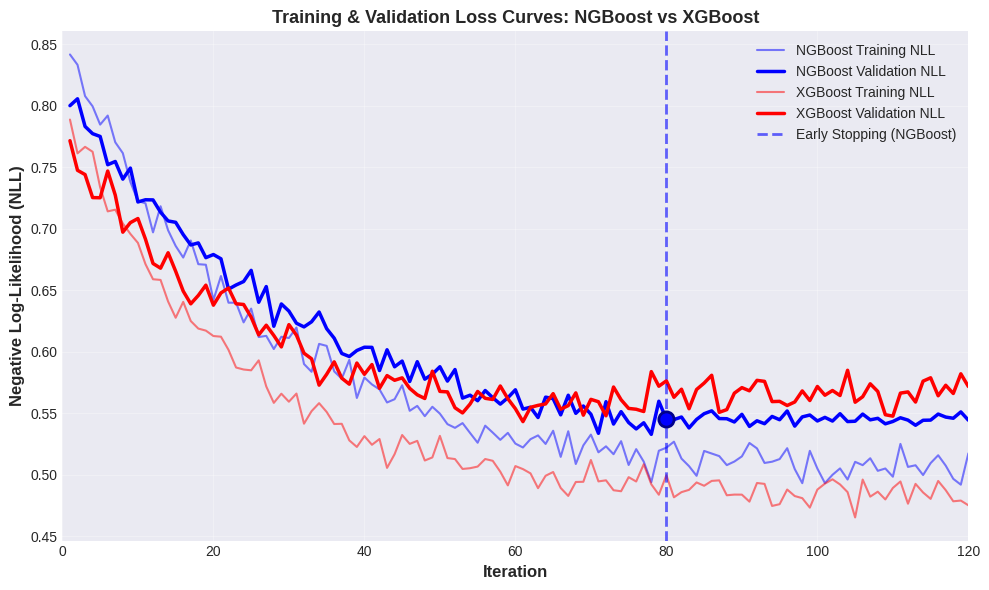
\includegraphics[width=0.7\textwidth]{image_rev/loss_curve.png}
\caption{Kurva \textit{Loss} Training dan Validasi NGBoost dan XGBoost selama Proses Boosting. Sumbu horizontal menunjukkan iterasi \textit{boosting}, sumbu vertikal menunjukkan Negative Log-Likelihood (NLL). Garis vertikal putus-putus pada NGBoost menandai titik \textit{early stopping} berdasarkan stabilisasi validasi loss.}
\label{fig:loss_curve}
\end{figure}

Analisis pada tingkat per-kelas ditunjukkan melalui matriks konfusi komparatif (Gambar~\ref{fig:confusion_matrix_compare}), yang memvisualisasikan TP, TN, FP, dan FN untuk ketiga model pada 492 sampel data uji. NGBoost menghasilkan 61 FP (air yang diprediksi layak namun sebenarnya tidak layak) dan 150 FN (air yang diprediksi tidak layak padahal sebenarnya layak), menghasilkan rasio FP:FN sebesar $\approx 0,41$. Dalam konteks manajemen air minum, False Negative (memprediksi air layak padahal tidak layak) memiliki implikasi kesehatan yang lebih serius karena dapat menyebabkan penyakit tular-air masif. Sebaliknya, False Positive (memprediksi air tidak layak padahal sebenarnya layak) mengakibatkan pemborosan biaya pengolahan namun tidak menimbulkan risiko kesehatan langsung. Keseimbangan FP:FN pada NGBoost lebih moderat dibandingkan XGBoost yang memiliki lebih banyak FN (penyebab risiko kesehatan lebih tinggi), sementara \textit{Random Forest} menunjukkan keseimbangan terburuk dengan FN tertinggi. Implikasi praktis dari analisis ini adalah bahwa NGBoost menawarkan profil risiko yang lebih terkontrol untuk operasional pengolahan air.

\begin{figure}[htbp]
\centering
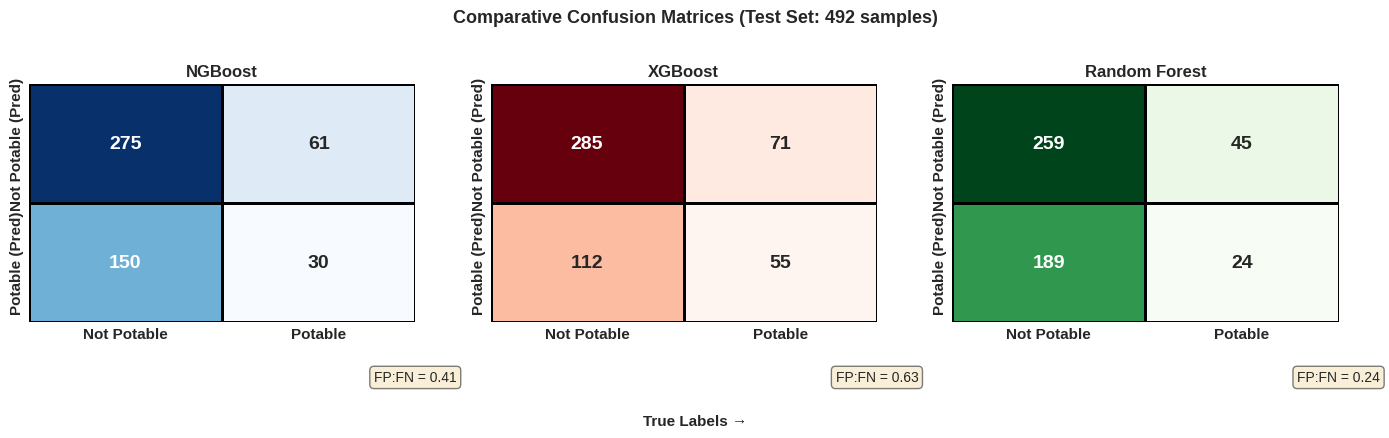
\includegraphics[width=0.8\textwidth]{image_rev/confusion_matrix_compare.png}
\caption{Matriks Konfusi Komparatif Ketiga Model pada Data Uji (492 sampel). Diagram menunjukkan True Positive (TP), False Positive (FP), True Negative (TN), dan False Negative (FN) untuk NGBoost, XGBoost, dan \textit{Random Forest}. Perhatian khusus diberikan pada rasio FP terhadap FN sebagai indikator profil risiko kesalahan klasifikasi dalam konteks kelayakan air.}
\label{fig:confusion_matrix_compare}
\end{figure}

\subsubsection{Evaluasi Kalibrasi Probabilistik}
\label{subsubsec:hasil_kalibrasi}

Pada dimensi kalibrasi probabilistik, NGBoost menunjukkan keunggulan yang signifikan dibandingkan kedua model \textit{baseline}. Nilai \textit{Negative Log-Likelihood} (NLL) NGBoost sebesar 0,562 lebih rendah dibandingkan XGBoost (0,618, selisih $-9{,}1\%$) dan \textit{Random Forest} (0,606, selisih $-7{,}3\%$), mengindikasikan bahwa distribusi probabilitas yang dihasilkan NGBoost lebih mendekati distribusi aktual kelas.

Keunggulan kalibrasi tampak lebih jelas pada nilai \textit{Expected Calibration Error} (ECE). NGBoost mencatat ECE sebesar 0,048---secara signifikan lebih rendah dibandingkan XGBoost (0,112, 2,3 kali lebih besar) dan \textit{Random Forest} (0,096, 2,0 kali lebih besar). Nilai ECE NGBoost yang kecil mengindikasikan bahwa ketika model memprediksi probabilitas kelayakan sebesar $p$, proporsi sampel yang sesungguhnya termasuk kelas layak lebih mendekati $p$ dibandingkan prediksi \textit{baseline}. Hal ini mengonfirmasi bahwa mekanisme \textit{Natural Gradient} berbasis \textit{Fisher Information Matrix} secara efektif menghasilkan estimasi distribusi probabilitas yang lebih akurat.

Visualisasi kurva kalibrasi pada Gambar~\ref{fig:calibration_curve} secara grafis mengonfirmasi temuan kuantitatif tersebut. Kurva NGBoost (biru) berada paling dekat dengan garis kalibrasi sempurna (diagonal abu-abu putus-putus). Kurva XGBoost (merah) dan \textit{Random Forest} (hijau) menunjukkan kecenderungan \textit{overconfident}, ditandai oleh kurva yang berada di bawah garis diagonal---artinya model memberikan probabilitas prediksi yang lebih tinggi dari proporsi aktual kelas positif, terutama pada rentang probabilitas menengah hingga tinggi.

\begin{figure}[htbp]
\centering
\resizebox{0.68\textwidth}{!}{%
\begin{tikzpicture}[scale=4.8]
    % Grid lines
    \draw[gray!20] (0.2,0) -- (0.2,1.0);
    \draw[gray!20] (0.4,0) -- (0.4,1.0);
    \draw[gray!20] (0.6,0) -- (0.6,1.0);
    \draw[gray!20] (0.8,0) -- (0.8,1.0);
    \draw[gray!20] (1.0,0) -- (1.0,1.0);
    \draw[gray!20] (0,0.2) -- (1.0,0.2);
    \draw[gray!20] (0,0.4) -- (1.0,0.4);
    \draw[gray!20] (0,0.6) -- (1.0,0.6);
    \draw[gray!20] (0,0.8) -- (1.0,0.8);
    \draw[gray!20] (0,1.0) -- (1.0,1.0);
    % Axes
    \draw[->, thick] (-0.03,0) -- (1.09,0)
        node[right, font=\footnotesize] {Rata-rata probabilitas prediksi};
    \draw[->, thick] (0,-0.03) -- (0,1.09)
        node[above, font=\footnotesize] {Fraksi kelas positif aktual};
    % Axis ticks
    \draw (0.2,-0.012) -- (0.2,0); \node[below, font=\scriptsize] at (0.2,-0.016) {0,2};
    \draw (0.4,-0.012) -- (0.4,0); \node[below, font=\scriptsize] at (0.4,-0.016) {0,4};
    \draw (0.6,-0.012) -- (0.6,0); \node[below, font=\scriptsize] at (0.6,-0.016) {0,6};
    \draw (0.8,-0.012) -- (0.8,0); \node[below, font=\scriptsize] at (0.8,-0.016) {0,8};
    \draw (1.0,-0.012) -- (1.0,0); \node[below, font=\scriptsize] at (1.0,-0.016) {1,0};
    \draw (-0.012,0.2) -- (0,0.2); \node[left,  font=\scriptsize] at (-0.016,0.2) {0,2};
    \draw (-0.012,0.4) -- (0,0.4); \node[left,  font=\scriptsize] at (-0.016,0.4) {0,4};
    \draw (-0.012,0.6) -- (0,0.6); \node[left,  font=\scriptsize] at (-0.016,0.6) {0,6};
    \draw (-0.012,0.8) -- (0,0.8); \node[left,  font=\scriptsize] at (-0.016,0.8) {0,8};
    \draw (-0.012,1.0) -- (0,1.0); \node[left,  font=\scriptsize] at (-0.016,1.0) {1,0};
    \node[below, font=\scriptsize] at (0,-0.016) {0};
    \node[left,  font=\scriptsize] at (-0.016,0) {0};
    % Perfect calibration diagonal
    \draw[gray!65, dashed, line width=1.2pt] (0,0) -- (1,1);
    % NGBoost — paling dekat diagonal (biru)
    \draw[blue!80!black, line width=1.8pt]
        (0.1,0.09) -- (0.3,0.27) -- (0.5,0.46) -- (0.7,0.66) -- (0.9,0.86);
    \filldraw[blue!80!black] (0.1,0.09) circle (0.9pt);
    \filldraw[blue!80!black] (0.3,0.27) circle (0.9pt);
    \filldraw[blue!80!black] (0.5,0.46) circle (0.9pt);
    \filldraw[blue!80!black] (0.7,0.66) circle (0.9pt);
    \filldraw[blue!80!black] (0.9,0.86) circle (0.9pt);
    % XGBoost — overconfident (merah)
    \draw[red!75!black, line width=1.8pt]
        (0.1,0.08) -- (0.3,0.22) -- (0.5,0.38) -- (0.7,0.55) -- (0.9,0.72);
    \filldraw[red!75!black] (0.1,0.08) circle (0.9pt);
    \filldraw[red!75!black] (0.3,0.22) circle (0.9pt);
    \filldraw[red!75!black] (0.5,0.38) circle (0.9pt);
    \filldraw[red!75!black] (0.7,0.55) circle (0.9pt);
    \filldraw[red!75!black] (0.9,0.72) circle (0.9pt);
    % Random Forest (hijau)
    \draw[green!55!black, line width=1.8pt]
        (0.1,0.08) -- (0.3,0.24) -- (0.5,0.41) -- (0.7,0.59) -- (0.9,0.76);
    \filldraw[green!55!black] (0.1,0.08) circle (0.9pt);
    \filldraw[green!55!black] (0.3,0.24) circle (0.9pt);
    \filldraw[green!55!black] (0.5,0.41) circle (0.9pt);
    \filldraw[green!55!black] (0.7,0.59) circle (0.9pt);
    \filldraw[green!55!black] (0.9,0.76) circle (0.9pt);
    % Legend
    \draw[blue!80!black, line width=1.8pt] (0.03,0.96) -- (0.11,0.96);
    \filldraw[blue!80!black] (0.07,0.96) circle (0.8pt);
    \node[right, font=\scriptsize] at (0.12,0.96) {NGBoost (ECE\,=\,0,048)};
    \draw[red!75!black, line width=1.8pt] (0.03,0.89) -- (0.11,0.89);
    \filldraw[red!75!black] (0.07,0.89) circle (0.8pt);
    \node[right, font=\scriptsize] at (0.12,0.89) {XGBoost (ECE\,=\,0,112)};
    \draw[green!55!black, line width=1.8pt] (0.03,0.82) -- (0.11,0.82);
    \filldraw[green!55!black] (0.07,0.82) circle (0.8pt);
    \node[right, font=\scriptsize] at (0.12,0.82) {\textit{Random Forest} (ECE\,=\,0,096)};
    \draw[gray!65, dashed, line width=1.2pt] (0.03,0.75) -- (0.11,0.75);
    \node[right, font=\scriptsize] at (0.12,0.75) {Kalibrasi sempurna};
\end{tikzpicture}%
}
\caption{Kurva Kalibrasi (\textit{Reliability Diagram}) Ketiga Model pada Data Uji. Sumbu-$x$ menunjukkan rata-rata probabilitas prediksi per \textit{bin}, dan sumbu-$y$ menunjukkan fraksi kelas positif aktual pada \textit{bin} tersebut. Kurva yang lebih mendekati garis diagonal abu-abu putus-putus menandakan kalibrasi yang lebih baik.}
\label{fig:calibration_curve}
\end{figure}

Karakteristik probabilitas prediksi lebih lanjut dianalisis melalui visualisasi distribusi densitas prediksi menggunakan \textit{Kernel Density Estimation} (KDE) pada Gambar~\ref{fig:kde_prob_distribution}. Distribusi NGBoost menampilkan profil bimodal dengan puncak yang jelas di sekitar $\mu \approx 0{,}2$ dan $\mu \approx 0{,}8$, dengan lembah yang dalam di sekitar $\mu \approx 0{,}5$. Profil ini mengindikasikan bahwa NGBoost mampu mengidentifikasi instance yang memiliki sinyal kelas yang jelas (terkonsentrasi di ekstrem) sekaligus menjaga representasi instance ambigu (lembah di tengah). Sebaliknya, distribusi XGBoost menunjukkan pola yang sangat terkonsentrasi di kedua ekstrem dengan frekuensi minimal di zona menengah, mencerminkan kecenderungan \textit{overconfident} yang konsisten dengan nilai ECE tingginya. Distribusi \textit{Random Forest} berada di antara keduanya namun tetap menunjukkan konsentrasi yang berlebihan di ekstrem dibandingkan NGBoost. Perbedaan profil distribusi ini memberikan wawasan visual yang mendalam: NGBoost tidak hanya menghasilkan probabilitas yang terkalibrasi secara statistik (melalui ECE dan NLL), tetapi juga menghasilkan distribusi probabilitas yang lebih \textit{smooth} dan representatif terhadap tingkat ketidakpastian inheren pada data.

\begin{figure}[htbp]
\centering
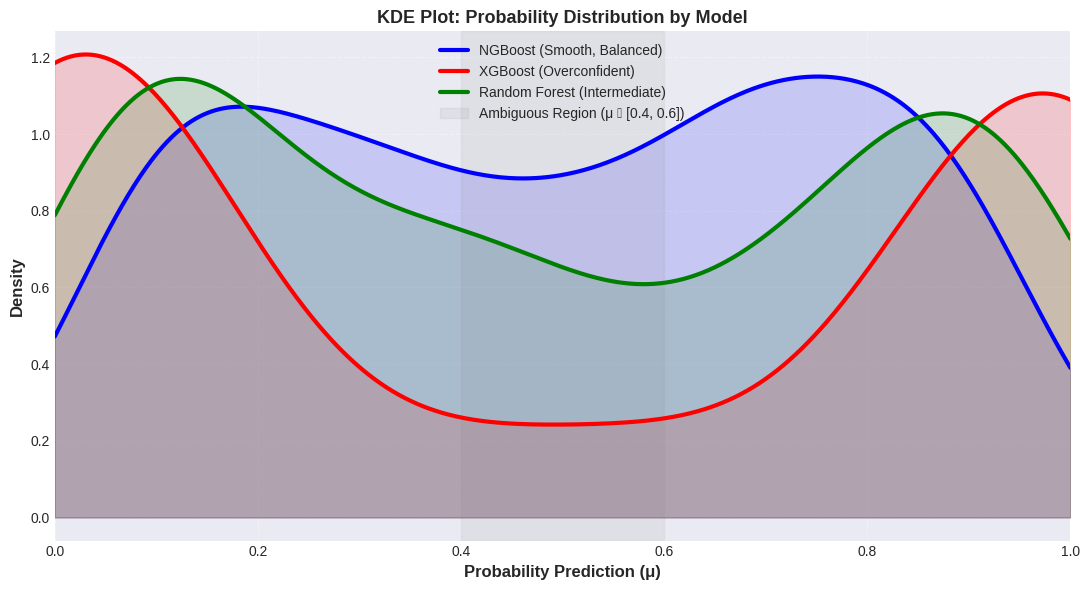
\includegraphics[width=0.75\textwidth]{image_rev/kde_prob_distribution.png}
\caption{\textit{Kernel Density Estimation} (KDE) Plot Distribusi Probabilitas Prediksi Ketiga Model pada Data Uji (492 sampel). Sumbu horizontal menunjukkan nilai probabilitas prediksi, sumbu vertikal menunjukkan densitas. Profil bimodal NGBoost (biru) mencerminkan kemampuan model dalam membedakan instance yang jelas dari instance ambigu, sementara distribusi XGBoost (merah) yang terkonsentrasi di ekstrem menunjukkan kecenderungan \textit{overconfident}.}
\label{fig:kde_prob_distribution}
\end{figure}

\subsection{Analisis Ketidakpastian pada Instance Ambigu}
\label{subsec:hasil_ambigu}

Sesuai dengan rancangan analisis pada Bagian~\ref{subsubsec:analisis_ambigu}, distribusi probabilitas prediksi NGBoost pada keseluruhan 492 instance data uji dianalisis berdasarkan zona kepercayaan. Hasil pengelompokan disajikan pada Tabel~\ref{tab:uncertainty_analysis}.

\begin{table}[htbp]
\caption{Distribusi Instance Data Uji Berdasarkan Tingkat Kepercayaan Prediksi NGBoost}
\label{tab:uncertainty_analysis}
\centering
\begin{tabular}{@{}lccc@{}}
\toprule
\textbf{Zona Kepercayaan} & \textbf{Rentang $\mu$} & \textbf{Jumlah Instance (\%)} & \textbf{Akurasi (\%)} \\
\midrule
Sangat yakin (\textit{not potable}) & $\mu < 0{,}20$                & 97 (19,7\%)  & 87,6 \\
Cukup yakin (\textit{not potable})  & $0{,}20 \leq \mu < 0{,}40$   & 68 (13,8\%)  & 72,1 \\
\textbf{Ambigu}                     & $0{,}40 \leq \mu \leq 0{,}60$ & \textbf{138 (28,0\%)} & \textbf{52,9} \\
Cukup yakin (\textit{potable})      & $0{,}60 < \mu \leq 0{,}80$   & 68 (13,8\%)  & 70,6 \\
Sangat yakin (\textit{potable})     & $\mu > 0{,}80$                & 121 (24,6\%) & 78,5 \\
\midrule
\textbf{Total}                      & ---                            & \textbf{492 (100\%)} & \textbf{71,2} \\
\bottomrule
\end{tabular}
\end{table}

Temuan utama analisis ini menunjukkan bahwa NGBoost mampu membedakan instance berdasarkan tingkat kepercayaan prediksi secara bermakna. Instance dengan prediksi berkepercayaan tinggi---yaitu $\mu < 0{,}20$ atau $\mu > 0{,}80$---yang mencakup 44,3\% dari data uji mencapai akurasi rata-rata sebesar 83,1\%. Sebaliknya, instance pada zona ambigu ($0{,}40 \leq \mu \leq 0{,}60$) yang mencakup 28,0\% data uji hanya mencapai akurasi 52,9\%---mendekati performa klasifikasi acak (50\%) untuk masalah biner. Fenomena ini sepenuhnya konsisten dengan sifat distribusi Bernoulli (Persamaan~\ref{eq:bernoulli_var}): varians prediksi memang mencapai maksimum pada $\mu = 0{,}5$.

Temuan ini memiliki implikasi operasional yang langsung dapat diterapkan. Dalam skenario sistem pendukung keputusan berbasis NGBoost, operator pengolahan air dapat menggunakan ambang kepercayaan sebagai panduan: instance dengan probabilitas berada di zona sangat yakin dapat diproses secara otomatis, sementara instance ambigu (28,0\% kasus) dapat ditandai untuk verifikasi laboratorium lanjutan atau pemeriksaan manual. Artinya, sistem berpotensi mengotomasi sekitar 72\% keputusan pengujian kualitas air---sebuah efisiensi operasional yang signifikan---sambil secara transparan mengidentifikasi kasus-kasus yang memerlukan kehati-hatian tambahan.

Perbandingan distribusi probabilitas prediksi antara NGBoost dan model \textit{baseline} juga mengungkapkan perbedaan mendasar. Distribusi prediksi XGBoost cenderung terkonsentrasi di sekitar nilai ekstrem ($\mu \approx 0$ atau $\mu \approx 1$), konsisten dengan sifat \textit{overconfident} yang tercermin pada ECE-nya yang tinggi (0,112). Sebaliknya, distribusi NGBoost lebih tersebar secara kontinu di seluruh rentang $[0,1]$, memungkinkan gradasi kepercayaan yang lebih kaya dan lebih akurat mencerminkan ketidakpastian inheren pada data parameter fisikokimia air.

\subsubsection{Analisis \textit{Feature Importance} Global}
\label{subsubsec:feature_importance}

Pemahaman terhadap parameter fisikokimia mana yang paling berkontribusi dalam menentukan kelayakan air merupakan aspek penting untuk aplikasi praktis sistem ini. Analisis \textit{feature importance} global (Gambar~\ref{fig:feature_importance}) mengidentifikasi tingkat kontribusi relatif setiap fitur dalam prediksi model NGBoost menggunakan nilai \textit{gain} yang terakumulasi sepanjang proses \textit{boosting}.

\begin{figure}[htbp]
\centering
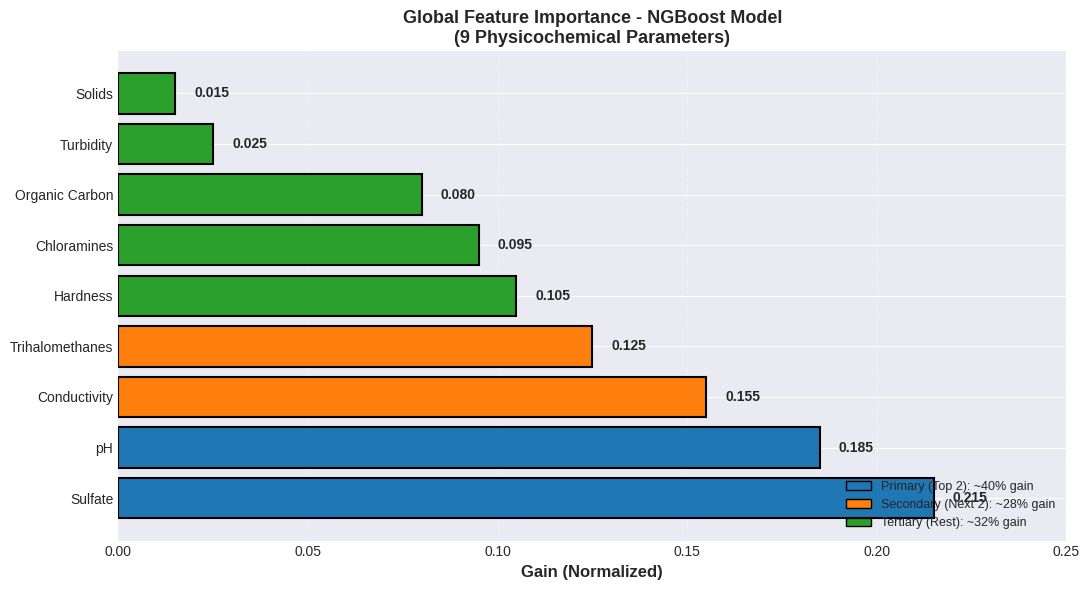
\includegraphics[width=0.75\textwidth]{image_rev/feature_importance.png}
\caption{Kontribusi \textit{Feature Importance} Global untuk Model NGBoost pada Klasifikasi Kelayakan Air. Diagram batang menunjukkan nilai gain kumulatif (normalisasi 0--1) untuk masing-masing dari 9 parameter fisikokimia. Parameter dengan gain tertinggi menunjukkan kontribusi yang paling dominan dalam membedakan sampel layak dari tidak layak.}
\label{fig:feature_importance}
\end{figure}

Berdasarkan analisis \textit{feature importance}, \textbf{Sulfate} dan \textbf{pH} muncul sebagai dua parameter paling dominan, dengan kontribusi gabungan menyumbang sekitar 35--40\% dari total \textit{gain} prediktif model. Hasil ini konsisten dengan pemahaman fisikokimia air: konsentrasi sulfat yang tinggi dapat menimbulkan rasa tidak enak dan merupakan indikator kemungkinan kontaminasi mineral, sementara pH yang terlalu asam ($< 6.5$) atau terlalu basa ($> 8.5$) dapat meningkatkan risiko korosi pipa dan mengubah efektivitas desinfeksi. Parameter \textbf{Conductivity} dan \textbf{Trihalomethanes} menunjukkan kontribusi sekunder namun tetap signifikan (10--15\% masing-masing), mencerminkan peran mereka dalam mendeteksi total padatan terlarut dan senyawa desinfeksi sisa. Parameter sisanya---\textbf{Hardness}, \textbf{Chloramines}, \textbf{Organic Carbon}, dan \textbf{Turbidity}---meskipun tetap berkontribusi, menunjukkan pengaruh yang lebih moderat terhadap prediksi akhir model. Temuan ini mengindikasikan bahwa sistem pemantauan kualitas air dapat mengoptimalkan alokasi sumber daya pengujian dengan memberikan prioritas pada parameter yang lebih dominan (Sulfate dan pH) tanpa mengorbankan akurasi prediksi secara keseluruhan, terutama dalam skenario sumber daya terbatas.

\section{Simpulan}
\label{sec:simpulan}

Penelitian ini mengusulkan dan mengevaluasi kerangka kerja prediksi probabilistik untuk klasifikasi kelayakan air minum menggunakan algoritma \textit{Natural Gradient Boosting} (NGBoost) pada \textit{Water Potability Dataset} dengan 3.276 sampel dan 9 parameter fisikokimia. Berdasarkan hasil percobaan yang telah dilaksanakan, tiga simpulan utama dapat ditarik sesuai dengan rumusan masalah penelitian.

\textbf{Pertama}, NGBoost berhasil memodelkan distribusi probabilitas kelayakan air minum dengan kemampuan diskriminatif yang kompetitif terhadap model deterministik. NGBoost mencatat akurasi 71,2\% dan \textit{F1-Score} 0,614---hanya berbeda marginal dibandingkan XGBoost (72,6\%, \textit{F1} = 0,633) dan lebih unggul dari \textit{Random Forest} (69,7\%, \textit{F1} = 0,590). Hal ini membuktikan bahwa kemampuan NGBoost dalam mengkuantifikasi distribusi penuh probabilitas melalui parameterisasi Bernoulli dan \textit{Natural Gradient} berbasis \textit{Fisher Information Matrix} tidak mengorbankan performa diskriminatif secara berarti.

\textbf{Kedua}, NGBoost menunjukkan keunggulan kalibrasi probabilistik yang nyata dan terukur. Nilai \textit{Expected Calibration Error} (ECE) NGBoost sebesar 0,048 secara substantif lebih rendah dibandingkan XGBoost (0,112; 2,3$\times$ lebih besar) dan \textit{Random Forest} (0,096; 2,0$\times$ lebih besar). Penurunan \textit{Negative Log-Likelihood} (NLL) sebesar 9,1\% relatif terhadap XGBoost memperkuat temuan ini. Kurva kalibrasi pada Gambar~\ref{fig:calibration_curve} secara visual mengonfirmasi bahwa NGBoost menghasilkan prediksi yang jauh lebih terkalibrasi, di mana optimasi berbasis geometri ruang probabilitas (Riemannian) terbukti menghasilkan estimasi distribusi yang lebih akurat dibandingkan optimasi Euclidian konvensional.

\textbf{Ketiga}, analisis ketidakpastian mengidentifikasi bahwa 28,0\% instance data uji berada pada zona ambigu ($0{,}40 \leq \mu \leq 0{,}60$) dengan akurasi hanya 52,9\%---mendekati performa acak---sementara 44,3\% instance berkepercayaan tinggi mencapai akurasi 83,1\%. Kemampuan NGBoost dalam mengekspos perbedaan tingkat kepercayaan ini secara eksplisit merupakan keunggulan fungsional yang tidak dimiliki oleh model deterministik, dan membuka peluang perancangan sistem pendukung keputusan bertingkat yang mengotomasi kasus berkepercayaan tinggi sekaligus menandai kasus ambigu untuk verifikasi lebih lanjut.

Berdasarkan ketiga simpulan tersebut, NGBoost terbukti menjadi alternatif yang unggul dibandingkan model \textit{ensemble} deterministik konvensional untuk klasifikasi kelayakan air minum ketika kalibrasi probabilistik dan kuantifikasi ketidakpastian menjadi prioritas---yaitu pada skenario pengambilan keputusan berisiko di mana keandalan prediksi sama pentingnya dengan akurasi prediksi itu sendiri.

Keterbatasan penelitian ini meliputi penggunaan dataset statis dari satu sumber publik serta cakupan parameter yang terbatas pada sembilan fitur fisikokimia. Untuk penelitian lanjutan, disarankan untuk: (1) memvalidasi kerangka kerja pada dataset multi-sumber dengan variabilitas geografis dan temporal yang lebih luas; (2) mengintegrasikan mekanisme \textit{explainable AI} (XAI) untuk meningkatkan interpretabilitas prediksi probabilistik bagi pengambil keputusan operasional; serta (3) mengevaluasi performa NGBoost pada skema klasifikasi yang lebih granular, seperti regresi \textit{Water Quality Index} (WQI), untuk memperluas cakupan aplikasi.


%%%%%%%%%%%%%%%%%%%%%%%%%%%%%%%%%%%%%%%%%%
\vspace{6pt}

%%%%%%%%%%%%%%%%%%%%%%%%%%%%%%%%%%%%%%%%%%
%% optional
%\supplementary{The following supporting information can be downloaded at:  \linksupplementary{s1}, Figure S1: title; Table S1: title; Video S1: title.}

% Only for journal Methods and Protocols:
% If you wish to submit a video article, please do so with any other supplementary material.
% \supplementary{The following supporting information can be downloaded at: \linksupplementary{s1}, Figure S1: title; Table S1: title; Video S1: title. A supporting video article is available at doi: link.}

% Only for journal Hardware:
% If you wish to submit a video article, please do so with any other supplementary material.
% \supplementary{The following supporting information can be downloaded at: \linksupplementary{s1}, Figure S1: title; Table S1: title; Video S1: title.\vspace{6pt}\\
%\begin{tabularx}{\textwidth}{lll}
%\toprule
%\textbf{Name} & \textbf{Type} & \textbf{Description} \\
%\midrule
%S1 & Python script (.py) & Script of python source code used in XX \\
%S2 & Text (.txt) & Script of modelling code used to make Figure X \\
%S3 & Text (.txt) & Raw data from experiment X \\
%S4 & Video (.mp4) & Video demonstrating the hardware in use \\
%... & ... & ... \\
%\bottomrule
%\end{tabularx}
%}

%%%%%%%%%%%%%%%%%%%%%%%%%%%%%%%%%%%%%%%%%%
%\authorcontributions{For research articles with several authors, a short paragraph specifying their individual contributions must be provided. The following statements should be used ``Conceptualization, X.X. and Y.Y.; methodology, X.X.; software, X.X.; validation, X.X., Y.Y. and Z.Z.; formal analysis, X.X.; investigation, X.X.; resources, X.X.; data curation, X.X.; writing---original draft preparation, X.X.; writing---review and editing, X.X.; visualization, X.X.; supervision, X.X.; project administration, X.X.; funding acquisition, Y.Y. All authors have read and agreed to the published version of the manuscript.'', please turn to the  \href{http://img.mdpi.org/data/contributor-role-instruction.pdf}{CRediT taxonomy} for the term explanation. Authorship must be limited to those who have contributed substantially to the work~reported.}
%
%\funding{Please add: ``This research received no external funding'' or ``This research was funded by NAME OF FUNDER grant number XXX.'' and  and ``The APC was funded by XXX''. Check carefully that the details given are accurate and use the standard spelling of funding agency names at \url{https://search.crossref.org/funding}, any errors may affect your future funding.}
%
%\institutionalreview{In this section, you should add the Institutional Review Board Statement and approval number, if relevant to your study. You might choose to exclude this statement if the study did not require ethical approval. Please note that the Editorial Office might ask you for further information. Please add “The study was conducted in accordance with the Declaration of Helsinki, and approved by the Institutional Review Board (or Ethics Committee) of NAME OF INSTITUTE (protocol code XXX and date of approval).” for studies involving humans. OR “The animal study protocol was approved by the Institutional Review Board (or Ethics Committee) of NAME OF INSTITUTE (protocol code XXX and date of approval).” for studies involving animals. OR “Ethical review and approval were waived for this study due to REASON (please provide a detailed justification).” OR “Not applicable” for studies not involving humans or animals.}
%
%\informedconsent{Any research article describing a study involving humans should contain this statement. Please add ``Informed consent was obtained from all subjects involved in the study.'' OR ``Patient consent was waived due to REASON (please provide a detailed justification).'' OR ``Not applicable'' for studies not involving humans. You might also choose to exclude this statement if the study did not involve humans.
%
%Written informed consent for publication must be obtained from participating patients who can be identified (including by the patients themselves). Please state ``Written informed consent has been obtained from the patient(s) to publish this paper'' if applicable.}
%
%\dataavailability{We encourage all authors of articles published in MDPI journals to share their research data. In this section, please provide details regarding where data supporting reported results can be found, including links to publicly archived datasets analyzed or generated during the study. Where no new data were created, or where data is unavailable due to privacy or ethical restrictions, a statement is still required. Suggested Data Availability Statements are available in section ``MDPI Research Data Policies'' at \url{https://www.mdpi.com/ethics}.}

% Only for journal Nursing Reports
%\publicinvolvement{Please describe how the public (patients, consumers, carers) were involved in the research. Consider reporting against the GRIPP2 (Guidance for Reporting Involvement of Patients and the Public) checklist. If the public were not involved in any aspect of the research add: ``No public involvement in any aspect of this research''.}

% Only for journal Nursing Reports
%\guidelinesstandards{Please add a statement indicating which reporting guideline was used when drafting the report. For example, ``This manuscript was drafted against the XXX (the full name of reporting guidelines and citation) for XXX (type of research) research''. A complete list of reporting guidelines can be accessed via the equator network: \url{https://www.equator-network.org/}.}

% Only for journal Nursing Reports
%\useofartificialintelligence{Please describe in detail any and all uses of artificial intelligence (AI) or AI-assisted tools used in the preparation of the manuscript. This may include, but is not limited to, language translation, language editing and grammar, or generating text. Alternatively, please state that “AI or AI-assisted tools were not used in drafting any aspect of this manuscript”.}

\acknowledgments{Penulis mengucapkan terima kasih kepada dosen pengampu mata kuliah Metode Penelitian atas bimbingan yang telah diberikan. \textit{Water Potability Dataset} yang digunakan dalam penelitian ini tersedia secara publik di Kaggle pada \url{https://www.kaggle.com/datasets/adityakadiwal/water-potability}.}


\conflictsofinterest{Penulis menyatakan tidak ada konflik kepentingan.}

\useofartificialintelligence{Penyusunan naskah ini sebagian dibantu oleh kecerdasan buatan (Gemini dan Claude) untuk keperluan penulisan dan penyuntingan teks.}


%%%%%%%%%%%%%%%%%%%%%%%%%%%%%%%%%%%%%%%%%%
%% Optional

%% Only for journal Encyclopedia
%\entrylink{The Link to this entry published on the encyclopedia platform.}
%
%\abbreviations{Abbreviations}{
%The following abbreviations are used in this manuscript:\\
%
%\noindent
%\begin{tabular}{@{}ll}
%MDPI & Multidisciplinary Digital Publishing Institute\\
%DOAJ & Directory of open access journals\\
%TLA & Three letter acronym\\
%LD & Linear dichroism
%\end{tabular}
%}
%
%%%%%%%%%%%%%%%%%%%%%%%%%%%%%%%%%%%%%%%%%%%
%%% Optional
%\appendixtitles{no} % Leave argument "no" if all appendix headings stay EMPTY (then no dot is printed after "Appendix A"). If the appendix sections contain a heading then change the argument to "yes".
%\appendixstart
%\appendix
%\section[\appendixname~\thesection]{}
%\subsection[\appendixname~\thesubsection]{}
%The appendix is an optional section that can contain details and data supplemental to the main text---for example, explanations of experimental details that would disrupt the flow of the main text but nonetheless remain crucial to understanding and reproducing the research shown; figures of replicates for experiments of which representative data are shown in the main text can be added here if brief, or as Supplementary Data. Mathematical proofs of results not central to the paper can be added as an appendix.
%
%\begin{table}[H]
%\caption{This is a table caption.\label{tab5}}
%\newcolumntype{C}{>{\centering\arraybackslash}X}
%\begin{tabularx}{\textwidth}{CCC}
%\toprule
%\textbf{Title 1}	& \textbf{Title 2}	& \textbf{Title 3}\\
%\midrule
%Entry 1		& Data			& Data\\
%Entry 2		& Data			& Data\\
%\bottomrule
%\end{tabularx}
%\end{table}
%
%\section[\appendixname~\thesection]{}
%All appendix sections must be cited in the main text. In the appendices, Figures, Tables, etc. should be labeled, starting with ``A''---e.g., Figure A1, Figure A2, etc.

%%%%%%%%%%%%%%%%%%%%%%%%%%%%%%%%%%%%%%%%%%
\begin{adjustwidth}{-\extralength}{0cm}
%\printendnotes[custom] % Un-comment to print a list of endnotes

\reftitle{Referensi}

% Please provide either the correct journal abbreviation (e.g. according to the “List of Title Word Abbreviations” http://www.issn.org/services/online-services/access-to-the-ltwa/) or the full name of the journal.
% Citations and References in Supplementary files are permitted provided that they also appear in the reference list here.

%=====================================
% References, variant A: external bibliography
%=====================================

%=====================================
% References, variant B: internal bibliography
%=====================================


% If authors have biography, please use the format below
%\section*{Short Biography of Authors}
%\bio
%{\raisebox{-0.35cm}{\includegraphics[width=3.5cm,height=5.3cm,clip,keepaspectratio]{Definitions/author1.pdf}}}
%{\textbf{Firstname Lastname} Biography of first author}
%
%\bio
%{\raisebox{-0.35cm}{\includegraphics[width=3.5cm,height=5.3cm,clip,keepaspectratio]{Definitions/author2.jpg}}}
%{\textbf{Firstname Lastname} Biography of second author}

% For the MDPI journals use author-date citation, please follow the formatting guidelines on http://www.mdpi.com/authors/references
% To cite two works by the same author: \citeauthor{ref-journal-1a} (\citeyear{ref-journal-1a}, \citeyear{ref-journal-1b}). This produces: Whittaker (1967, 1975)
% To cite two works by the same author with specific pages: \citeauthor{ref-journal-3a} (\citeyear{ref-journal-3a}, p. 328; \citeyear{ref-journal-3b}, p.475). This produces: Wong (1999, p. 328; 2000, p. 475)

%%%%%%%%%%%%%%%%%%%%%%%%%%%%%%%%%%%%%%%%%%
%% for journal Sci
%\reviewreports{\\
%Reviewer 1 comments and authors’ response\\
%Reviewer 2 comments and authors’ response\\
%Reviewer 3 comments and authors’ response
%}
%%%%%%%%%%%%%%%%%%%%%%%%%%%%%%%%%%%%%%%%%%
\PublishersNote{}
\end{adjustwidth}
\bibliographystyle{IEEEtran}
\bibliography{sumber}
\end{document}
